\documentclass[8pt, a4paper]{extarticle}

\usepackage{enumerate, amsmath, amsthm, amssymb, cancel, mathtools}

\usepackage[a4paper, left=0.7cm, right=0.7cm, top=0.7cm, bottom=0.7cm, landscape]{geometry}

\usepackage{algorithm}
\usepackage{booktabs} 
\usepackage{hyperref}
\usepackage{array}
\usepackage{svg}
\usepackage{algpseudocode}
\usepackage{tikz}
\usepackage{forest}
\usepackage[stretch=10,shrink=20]{microtype}
\usepackage{anyfontsize}
\usepackage{titlesec}
\usepackage{multicol}
\usepackage{bm}
\usepackage{xcolor}
\usepackage{enumitem}
\usepackage{mathrsfs}
\usepackage{soul}
\usepackage{amsmath}
\usepackage{booktabs}
\usepackage{caption}

\usepackage{anyfontsize}

\titleformat{\section}
  {\fontsize{9pt}{11pt}\selectfont\bfseries}
  {\thesection}{1em}{}

\titleformat{\subsection}
  {\fontsize{8pt}{10pt}\selectfont\bfseries}
  {\thesubsection}{1em}{}

\titlespacing*{\section}
  {0pt}{1.5ex}{0.8ex}

\titlespacing*{\subsection}
  {0pt}{1.2ex}{0.6ex}


\usepackage{tcolorbox}


\author{Timofey Shatnyy}

\linespread{1.3}

\newtcbox{\tsLabelYellow}{
    on line,
    colback=yellow!100,
    colframe=yellow!0,
    arc=3pt,
    boxrule=0pt,
    left=0pt,right=0pt,top=-1pt,bottom=-1pt
}

\newtcbox{\tsLabelOrange}{
    on line,
    colback=orange!55,
    colframe=orange!0,
    arc=3pt,
    boxrule=0pt,
    left=0pt,right=0pt,top=-1pt,bottom=-1pt
}

\newtcbox{\tsLabelBlue}{
    on line,
    colback=blue!45,
    colframe=blue!0,
    arc=3pt,
    boxrule=0pt,
    left=0pt,right=0pt,top=-1pt,bottom=-1pt
}

\newtcbox{\tsLabelLightBlue}{
    on line,
    colback=blue!25,
    colframe=blue!0,
    arc=3pt,
    boxrule=0pt,
    left=0pt,right=0pt,top=-1pt,bottom=-1pt
}

\newtcbox{\tsLabelGreen}{
    on line,
    colback=green!55,
    colframe=green!0,
    arc=3pt,
    boxrule=0pt,
    left=0pt,right=0pt,top=-1pt,bottom=-1pt
}

\newtcbox{\tsLabelRed}{
    on line,
    colback=red!55,
    colframe=red!0,
    arc=3pt,
    boxrule=0pt,
    left=0pt,right=0pt,top=-1pt,bottom=-1pt
}

\newcommand{\tsV}[1]{
    \mathbf{#1}
}


\newcommand{\tsVec}[1]{
    \mathbf{#1}
}

\newcommand{\tsB}[1]{
    \{#1\}
}


\newcommand{\tsS}[1]{
    \mathbb{#1}
}

\newcommand{\tsIdea}[2]{
    \tsLabelRed{\textbf{#1:}} \(\tsPoint\)#2
}

\newcommand{\tsThe}[2]{
    \tsLabelYellow{\textbf{T #1:}} \(\tsPoint\)#2
}

\newcommand{\tsDef}[2]{
    \tsLabelOrange{\textbf{D #1:}} \(\tsPoint\)#2
}

\newcommand{\tsLem}[2]{
    \tsLabelBlue{\textbf{L #1:}}  \(\tsPoint\)#2
}

\newcommand{\tsCor}[2]{
    \tsLabelGreen{\textbf{C #1:}}  \(\tsPoint\)#2
}

\newcommand{\tsProp}[2]{
    \tsLabelLightBlue{\textbf{P #1:}}  \(\tsPoint\)#2
}

\newcommand{\tsPoint}[0]{
    \\ \bullet
}


\begin{document}
\begin{multicols}{3}
    {\fontsize{6}{7}\selectfont
        \setcounter{section}{2}
        \section{Set, Relations, and Functions}
        \subsection{Sets}
\tsDef{3.2 (Equal sets)}{
    For sets $A$ and $B$,
    \(
    A = B \;\Longleftrightarrow\; \forall x \,(x \in A \iff x \in B).
    \)
}
\newline
\tsLem{3.1 (Equality of set elemetns and ord. pairs)}{
    For any sets $A$ and $B$,
    \(
    \{A\} = \{B\} \;\Longrightarrow\; A = B.
    \)
    \\
    \textbf{Ordered pairs:}
    \(
    (a,b) = (c,d) \;\Longleftrightarrow\; a = c \;\wedge\; b = d.
    \)
    \\
    \textbf{Odered pairs via sets:}
    \(
    (a,b) := \bigl\{ \{a\}, \{a,b\} \bigr\}.
    \)
}
\newline
\tsDef{3.3 (Subset)}{
    \(
    A \subseteq B \;\Longleftrightarrow\; \forall x \,(x \in A \Rightarrow x \in B).
    \)
}
\newline
\tsLem{3.2 (Sets equality and subsets)}{
    \(
    A = B \;\Longleftrightarrow\; (A \subseteq B) \wedge (B \subseteq A).
    \)
    Equivalently: \\
    \(
    \forall x \,\bigl((x \in A \Rightarrow x \in B) \wedge (x \in B \Rightarrow x \in A)\bigr)
    \;\Leftrightarrow\;
    \forall x \,(x \in A \iff x \in B).
    \)
}
\newline
\tsLem{3.3 (Transitivity of subsets)}{
    For all sets $A,B,C$,
    \(
    A \subseteq B \;\wedge\; B \subseteq C \;\Longrightarrow\; A \subseteq C.
    \)
}
\newline
\tsDef{3.4 (Union and Intersection)}{
    \(
    A \cup B := \{x \mid x \in A \vee x \in B\},
    \)
    \(
    A \cap B := \{x \mid x \in A \wedge x \in B\}.
    \)
    \\
    \textbf{Families of Sets:}
    Let $\mathcal{A}$ be a set of sets:\\
    \(
    \bigcap \mathcal{A} := \{x \mid x \in A \text{ for all } A \in \mathcal{A}\},
    \)
    \(
    \bigcup \mathcal{A} := \{x \mid x \in A \text{ for some } A \in \mathcal{A}\}.
    \)
    % \\
    % \textbf{Example:}
    % \\
    % \(
    % \mathcal{A} = \bigl\{\{a,b,c\}, \{a,c\}, \{a,b,c,f\}, \{a,c,d\}\bigr\},
    % \)
    % \\
    % \(
    % \bigcup \mathcal{A} = \{a,b,c,d,e,f\},
    % \qquad
    % \bigcap \mathcal{A} = \{a,c\}.
    % \)
    \\
    If $I$ is an index set and $\mathcal{A} = \{A_i \mid i \in I\}$, then
    \(
    \bigcap_{i \in I} A_i,
    \
    \bigcup_{i \in I} A_i.
    \)
}
\newline
\tsDef{3.5 (Set Difference)}{
    The difference of sets $B$ and $A$ is
    \(
    B \setminus A := \{x \in B \mid x \notin A\}.
    \)
}
\newline
\tsDef{3.6 (Empty Set)}{
    A set is called \emph{empty} if it contains no elements:
    \(
    \forall x \,(x \notin A).
    \)
}
\newline
\tsLem{3.5 (Uniqueness of an empty set)}{
    There is exactly \textbf{one} empty set, denoted $\varnothing$ or $\{\}$.
}
\newline
\tsLem{3.6 (Empty set is a subset of every set)}{
    The empty set is a subset of every set:
    \(
    \forall A \;(\varnothing \subseteq A).
    \)
    \\
    \textbf{Construction of natural numbers:}
    \(
    S(n) := n \cup \{n\} \ \text{(rec. sucsessor)}.
    \)
}
\newline
\tsDef{3.7 (Power Set)}{
    The power set of a set $A$, denoted $\mathcal{P}(A)$, is the set of all subsets of $A$:
    \(
    \mathcal{P}(A) := \{S \mid S \subseteq A\}.
    \)
    If $|A| = k$, then
    \(
    |\mathcal{P}(A)| = 2^k.
    \)
    In particular, for a set with $k$ elements, each element may be
    \emph{included} or \emph{excluded}, giving
    \(
    2 \times 2 \times \cdots \times 2 = 2^k
    \)
    possible subsets. Think of bit-mask of set elements.
    % \\
    % \textbf{Example (bit-mask intuition for $\{a,b\}$):}
    % \(
    % {\scriptsize
    %         \begin{array}{ccl}
    %             00 & \longleftrightarrow & \varnothing \\
    %             01 & \longleftrightarrow & \{b\}       \\
    %             10 & \longleftrightarrow & \{a\}       \\
    %             11 & \longleftrightarrow & \{a,b\}
    %         \end{array}
    %     }
    % \)
    % \subsection*{Counting Principle}
    % If a process has:
    % \begin{itemize}[noitemsep, topsep=0pt]
    %     \item $a$ choices for step 1,
    %     \item $b$ choices for step 2,
    %     \item $c$ choices for step 3,
    % \end{itemize}
    % then the total number of outcomes is
    % \(
    % a \times b \times c.
    % \)
}
% \newline

        \subsection{Relations}
\tsDef{3.8 (Cartesian product)}{
    The Cartesian product $A \times B$ of sets $A$ and $B$ is the set of all ordered pairs with first component from $A$ and second from $B$:
    \(
    A \times B := \{(a,b) \mid a \in A,\ b \in B\}.
    \)
    The cardinality satisfies
    \(
    |A \times B| = |A| \cdot |B|.
    \)
    \\
    \textbf{More generally:}
    \(
    \mathop{\scalebox{1.6}{$\times$}}_{i=1}^k A_i
    :=
    \{(a_1,\dots,a_k) \mid a_i \in A_i \text{ for } 1 \le i \le k\}.
    \)
    \\
    The Cartesian product is \emph{not associative}, since elements are ordered tuples.
    % \\
    % \textbf{Connection to power sets:}
    % \\
    % If
    % \(
    % A = \{a,b,c\}, \ |A|=3,
    % \)
    % then each element may be either \emph{in} or \emph{out}, giving
    % \(
    % \{0,1\}^3 = \{0,1\} \times \{0,1\} \times \{0,1\},
    % \)
    % which represents all subsets of $A$.
    \\
    \textbf{Example:}
    \\
    \(
    A_1 = \{0,1\}, \ A_2 = \{d,e\},
    \)
    \(
    A_1 \times A_2 = \{(0,d),(0,e),(1,d),(1,e)\}.
    \)
}
\newline
\tsDef{3.9 (Relation)}{
    A (binary) relation $\rho$ from a set $A$ to a set $B$ is a subset of $A \times B$.
    \\
    If $A=B$, then $\rho$ is called a relation \emph{on} $A$.
    \\
    \textbf{Notation:}
    \(
    (a,b) \in \rho \;\Rightarrow\; a \,\rho\, b,
    \
    (a,b) \notin \rho \;\Rightarrow\; a \not\!\rho\, b.
    \)
    \\
    For any set $S$, any subset $\rho \subseteq S \times S$ is a relation on $S$.
    \\
    There are
    \(
    2^{n^2}
    \)
    relations on a set of cardinality $n$, since
    \(
    |S \times S| = n^2
    \ \text{and} \
    |\mathcal{P}(S \times S)| = 2^{n^2}.
    \)
    \\
    % \textbf{Relations as Matrices:}
    % \\
    % Relations can be represented by $0$–$1$ matrices, analogous to adjacency matrices for graphs. Combining relations using set operations
    % \(
    % \cap,\ \cup,\ \setminus
    % \)
    % corresponds to applying logical operations
    % \(
    % \wedge,\ \vee,\ \neg
    % \)
    % entrywise to matrices.
    % \\
    \textbf{Examples on $\mathbb{Z}$:}
    \begin{itemize}[noitemsep, topsep=-3pt]
        \item $\leq \;\cup\; \geq$ is the complete relation $\mathbb{Z} \times \mathbb{Z}$.
        \item $\leq \;\cap\; \geq$ is the identity relation:
              \(
              \{(a,a) \mid a \in \mathbb{Z}\}.
              \)
    \end{itemize}
}
\tsDef{3.11 (Inverse Relation)}{
    The inverse relation of $\rho$ is
    \(
    \rho^{-1} := \{(b,a) \mid (a,b) \in \rho\}.
    \)
    \\
    Equivalently,
    \(
    b \,\rho^{-1}\, a \;\Longleftrightarrow\; a \,\rho\, b.
    \)
    \\
    % \textbf{Interpretations:}
    % \begin{itemize}[noitemsep, topsep=-3pt]
    %     \item In graphs: reversing all edge directions.
    %     \item In matrices: taking the transpose.
    % \end{itemize}
}
\tsDef{3.12 (Composition of Relations)}{
    Let $\rho \subseteq A \times B$ and $\sigma \subseteq B \times C$.
    The composition $\sigma \circ \rho$ is defined by
    \(
    \sigma \circ \rho
    :=
    \{(a,c) \mid \exists b \ ((a,b) \in \rho \wedge (b,c) \in \sigma)\}.
    \)
    Composition is associative:
    \(
    \rho \circ (\sigma \circ \tau) = (\rho \circ \sigma) \circ \tau.
    \)
}
\newline
\tsLem{3.8 (Inverse of relation composition)}{
    Let $\rho$ be a relation from $A$ to $B$ and $\sigma$ a relation from $B$ to $C$.
    Then
    \(
    (\sigma \circ \rho)^{-1} = \rho^{-1} \circ \sigma^{-1}.
    \)
}

        \subsection{Properties of Relations}
\begin{center}
    \renewcommand{\arraystretch}{1.4}
    \begin{tabular}{lccc}
        \toprule
        \textbf{Name} & \textbf{Formula}                             & \textbf{Set} & \textbf{Example} \\
        \midrule
        Reflexive
                      & $a\rho a$
                      & $\mathrm{id} \subseteq \rho$
                      & $\mathrm{id},\, \geq$                                                          \\

        Irreflexive
                      & $\neg(a\rho a)$
                      & $\mathrm{id} \cap \rho = \varnothing$
                      & $\neq,\, >$                                                                    \\

        Symmetric
                      & $a\rho b \iff b\rho a$
                      & $\rho = \hat{\rho}$
                      & $\mathrm{id},\, \equiv\ (\mathrm{mod}\ m)$                                     \\

        Antisymmetric
                      & $a\rho b \wedge b\rho a \rightarrow a=b$
                      & $\rho \cap \hat{\rho} \subseteq \mathrm{id}$
                      & $\geq,\, \mid$                                                                 \\

        Transitive
                      & $a\rho b \wedge b\rho c \rightarrow a\rho c$
                      & $\rho^{2} \subseteq \rho$
                      & $\equiv\ (\mathrm{mod}\ m),\, >$                                               \\
        \bottomrule
    \end{tabular}
\end{center}
% \tsDef{3.13 (Reflexive Relation)}{
%     A relation $\rho$ on a set $A$ is called \emph{reflexive} if
%     \(
%     \forall a \in A,\ a \,\rho\, a.
%     \)
%     \\
%     Equivalently,
%     \(
%     \mathrm{id}_A \subseteq \rho.
%     \)
% }
% \newline
% \tsDef{3.14 (Irreflexive Relation)}{
%     A relation $\rho$ on a set $A$ is called \emph{irreflexive} if
%     \(
%     \forall a \in A,\ a \not\!\rho\, a.
%     \)
%     \\
%     Equivalently,
%     \(
%     \rho \cap \mathrm{id}_A = \varnothing.
%     \)
% }
% \newline
% \tsDef{3.15 (Symmetric Relation)}{
%     A relation $\rho$ on a set $A$ is called \emph{symmetric} if
%     \(
%     a \,\rho\, b \;\Leftrightarrow\; b \,\rho\, a
%     \ \forall a,b \in A.
%     \)
%     \\
%     Equivalently,
%     \(
%     \rho = \rho^{-1}.
%     \)
%     \\
%     Interpretations:
%     \begin{itemize}[noitemsep, topsep=-3pt]
%         \item In matrix form: the matrix of $\rho$ is symmetric.
%         \item In graphs: the graph is undirected (possibly with loops).
%     \end{itemize}
% }
% \tsDef{3.16 (Antisymmetric Relation)}{
%     A relation $\rho$ on a set $A$ is called \emph{antisymmetric} if
%     \(
%     (a \,\rho\, b \;\wedge\; b \,\rho\, a) \;\Rightarrow\; a = b
%     \ \forall a,b \in A.
%     \)
%     \\
%     Equivalently,
%     \(
%     \rho \cap \rho^{-1} \subseteq \mathrm{id}_A.
%     \)
% }
% \newline
% \tsDef{3.17 (Transitive Relation)}{
%     A relation $\rho$ on a set $A$ is called \emph{transitive} if
%     \(
%     (a \,\rho\, b \;\wedge\; b \,\rho\, c) \;\Longrightarrow\; a \,\rho\, c.
%     \)
% }
% \newline
% \newline
\tsLem{3.9 (Transitivity and relation composition)}{
    A relation $\rho$ is transitive if and only if
    \(
    \rho^2 \subseteq \rho,
    \)
    where $\rho^2 = \rho \circ \rho$.
}
\newline
\tsDef{3.18 (Transitive Closure)}{
    The \emph{transitive closure} of a relation $\rho$ on a set $A$, denoted $\rho^{*}$, is defined by
    \(
    \rho^{*} := \bigcup_{n \in \mathbb{N}_{>0}} \rho^{n}.
    \)
    For a transitive relation \(\rho\) we have \(\rho^2 \subseteq \rho\).
}
\newline

        \subsection{Equivalence Relation}
\tsDef{3.19 (Equivalence Relation)}{
    An equivalence relation on a set $A$ is a relation that is
    \emph{reflexive}, \emph{symmetric}, and \emph{transitive}.
}
\newline
\tsDef{3.20 (Equivalence Class)}{
    Let $\theta$ be an equivalence relation on a set $A$, and let $a \in A$.
    The \emph{equivalence class} of $a$ is
    \(
    [a]_{\theta} := \{\, b \in A \mid b \,\theta\, a \,\}.
    \)
    \\
    \textbf{Example:} (congruence modulo $3$ on $\mathbb{Z}$):
    \(
    [0] = \{\dots,-6,-3,0,3,6,\dots\},
    \)
    \(
    [1] = \{\dots,-5,-2,1,4,7,\dots\},
    \)
    \(
    [2] = \{\dots,-4,-1,2,5,8,\dots\}.
    \)
}
\newline
\tsLem{3.10 (Intersection of equivalence relaltions)}{
    The intersection of two equivalence relations on the same set is an equivalence relation.
}
\newline
\tsDef{3.21 (Partition)}{
    A \emph{partition} of a set $A$ is a family $\{S_i \mid i \in I\}$ of subsets of $A$
    such that
    \(
    S_i \cap S_j = \varnothing \ (i \neq j),
    \
    \bigcup_{i \in I} S_i = A.
    \)
}
\newline
\tsDef{3.22 (Quotient Set)}{
    Let $\theta$ be an equivalence relation on a set $A$.
    The set of equivalence classes is denoted by
    \(
    A / \theta := \{ [a]_{\theta} \mid a \in A \},
    \)
    and is called the \emph{quotient set} of $A$ modulo $\theta$.
}
\newline
\tsThe{3.11 (Set of equiv. classes forms a partition of a set)}{
    Let $\theta$ be an equivalence relation on a set $A$.
    Then the set $A/\theta$ of equivalence classes forms a partition of $A$.
}
\newline

        \subsection{Partial Order Relations}
\tsDef{3.23 (Partial Order)}{
    A \emph{partial order} on a set $A$ is a relation that is
    \emph{reflexive}, \emph{antisymmetric}, and \emph{transitive}.
    \\
    A set equipped with a partial order $\preceq$ is called a
    \emph{partially ordered set} (poset), denoted $(A,\preceq)$.
    \\
    \textbf{Examples:}
    \(
    (\mathcal{P}(A), \subseteq) \text{ is a poset},
    \)
    \(
    (\mathbb{N}_{\ge 0}, \mid) \text{ is a poset},
    \)
    \(
    (\mathbb{Z}, \preceq) \text{ is a poset}.
    \)
    \\
    Note:
    \(
    a \prec b \;\Longleftrightarrow\; a \preceq b \;\wedge\; a \ne b.
    \)
}
\newline
\tsDef{3.24 (Comparable Elements)}{
    In a poset $(A,\preceq)$, two elements $a,b \in A$ are called \emph{comparable} if
    \(
    a \preceq b \ \text{or} \ b \preceq a.
    \)
    Otherwise, they are called \emph{incomparable}.
}
\newline
\tsDef{3.25 (Total Order)}{
    Let $(A,\preceq)$ be a poset.
    If any two elements of $A$ are comparable, then $A$ is called a
    \emph{totally ordered set} (or \emph{linearly ordered}) by $\preceq$.
    \\
    \textbf{Examples:}
    \(
    (\mathbb{Z},\le) \ \text{and} \ (\mathbb{Z},\ge)
    \)
    are totally ordered,
    \((\mathcal{P}(A),\subseteq)\) is not totally ordered if $|A|\ge 2$,
    \(
    (\mathbb{N},\mid)
    \) is not totally ordered
}
\newline
\tsDef{3.26 (Covering Relation)}{
    In a poset $(A,\preceq)$, an element $b$ \emph{covers} $a$ if: \\
    \(
    a \prec b \ \text{and there is no } c \text{ with } a \prec c \prec b
    \)
    between $a$ and $b$.
}
\newline
\tsDef{3.27 (Hasse Diagram)}{
    The \emph{Hasse diagram} of a finite poset $(A,\preceq)$ is the directed graph
    whose vertices are the elements of $A$, and where there is an edge from
    $a$ to $b$ if and only if $b$ covers $a$.
    \\
    \textbf{Example:}
    \(
    (\mathcal{P}(\{a,b,c\}),\subseteq).
    \)
}
\newline
\tsDef{3.28 (Direct product of posets)}{
    Let $(A,\preceq_A)$ and $(B,\preceq_B)$ be posets.
    The direct product poset $(A\times B,\le)$ is defined by
    \(
    (a_1,b_1)\le (a_2,b_2)
    \;\Longleftrightarrow\;
    a_1 \preceq_A a_2 \;\wedge\; b_1 \preceq_B b_2.
    \)
}
\newline
\tsThe{3.12 (Direct product of posets is a poset)}{
    If $(A,\preceq_A)$ and $(B,\preceq_B)$ are posets, then
    \(
    (A,\preceq_A)\times(B,\preceq_B)
    \)
    is a partially ordered set.
}
\newline
\tsThe{3.13 (Lexicographic Order)}{
    For posets $(A,\preceq_A)$ and $(B,\preceq_B)$, the relation
    \(
    (a_1,b_1)\le_{\text{lex}}(a_2,b_2)
    \;\Longleftrightarrow\;
    a_1\prec a_2 \;\vee\; (a_1=a_2 \wedge b_1\preceq_B b_2)
    \)
    defines a partial order on $A\times B$. It is called the lexicographic order.
}
\newline
\tsDef{3.29 (Bounds)}{
    Let $(A,\preceq)$ be a poset and $S\subseteq A$. For $a\in A$:
    $\tsPoint$ $a$ is \emph{minimal / maximal} if there is no $b\in A$
    with $b\prec a$ / $b\succ a$.
    $\tsPoint$ $a$ is the \emph{least / greatest element} of $A$ if
    \(
    a\preceq b \ / \ a\succeq b \ \forall b\in A.
    \)
    $\tsPoint$ $a$ is a \emph{lower / upper bound} of $S$ if
    \(
    a\preceq b \ / \ a\succeq b \ \forall b\in S.
    \)
    $\tsPoint$ $a$ is the \emph{greatest lower bound} /
    \emph{least upper bound} of $S$ if it is respectively the
    greatest / least among all lower / upper bounds of $S$.
}
\newline
\tsDef{3.30 (Well-Ordered Set)}{
    A poset $(A,\preceq)$ is \emph{well-ordered} if it is totally ordered and
    every nonempty subset of $A$ has a least element.
    \(\tsPoint\) Every subset of a well-ordered set is also well-ordered.
}
\newline
\tsDef{3.31 (Meet and Join)}{
    Let $(A,\preceq)$ be a poset and $a,b\in A$.
    \(\tsPoint\) If $a$ and $b$ have a greatest lower bound, it is called the
    \emph{meet} and denoted $a\wedge b$.
    \(\tsPoint\) If $a$ and $b$ have a least upper bound, it is called the
    \emph{join} and denoted $a\vee b$.
}
\newline
\tsDef{3.32 (Lattice)}{
    A poset $(A,\preceq)$ in which every pair of elements has both a meet and a
    join is called a \emph{lattice}.
}
\vspace{-1.5\baselineskip}
\begin{center}
    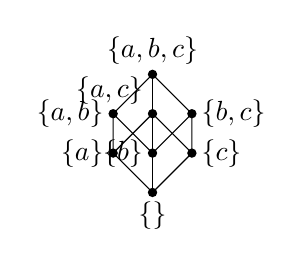
\begin{tikzpicture}[
            dot/.style={circle, fill=black, inner sep=1.2pt},
            lab/.style={font=\bfseries}
        ]

        % coordinates
        \coordinate (top) at (0,1.5);
        \coordinate (ab)  at (-0.5,1);
        \coordinate (ac)  at (0,1);
        \coordinate (bc)  at (0.5,1);

        \coordinate (a)   at (-0.5,0.5);
        \coordinate (b)   at (0,0.5);
        \coordinate (c)   at (0.5,0.5);

        \coordinate (bot) at (0,0);

        % edges (cover relations)
        \draw (top) -- (ab) -- (a) -- (bot);
        \draw (top) -- (bc) -- (c) -- (bot);
        \draw (top) -- (ac) -- (b) -- (bot);

        \draw (ab) -- (b);
        \draw (ac) -- (a);
        \draw (ac) -- (c);
        \draw (bc) -- (b);

        % dots
        \node[dot] at (top) {};
        \node[dot] at (ab)  {};
        \node[dot] at (ac)  {};
        \node[dot] at (bc)  {};
        \node[dot] at (a)   {};
        \node[dot] at (b)   {};
        \node[dot] at (c)   {};
        \node[dot] at (bot) {};

        % labels
        \node[lab, above]      at (top) {$\{a,b,c\}$};

        \node[lab, left]       at (ab)  {$\{a,b\}$};
        \node[lab, above left] at (ac)  {$\{a,c\}$};
        \node[lab, right]      at (bc)  {$\{b,c\}$};

        \node[lab, left]       at (a)   {$\{a\}$};
        \node[lab, left]      at (b)   {$\{b\}$};
        \node[lab, right]      at (c)   {$\{c\}$};

        \node[lab, below]      at (bot) {$\{\}$};
    \end{tikzpicture}
    \vspace{-0.7\baselineskip}
    \captionof{figure}{
        Lattice of the poset $(\mathcal{P}(S), \subseteq)$.
        \\
        Minimal, Least: \(\{\}\), Maximal, Greatest: \(\{\{a,b,c\}\}\).
    }
\end{center}
        \subsection{Functions}
\tsDef{3.33 (Function)}{
    A function $f:A\to B$ from domain $A$ to codomain $B$ is a relation from
    $A$ to $B$ such that:
    \(\tsPoint\) For every $a\in A$ there exists $b\in B$ with $a\,f\,b$
    (totality).
    \(\tsPoint\) For all $a\in A$ and $b,b'\in B$,
    \(
    a\,f\,b \wedge a\,f\,b' \;\Longrightarrow\; b=b'
    \)
    (well-definedness).
    We write $f(a)=b$.
}
\newline
\tsDef{3.34 (Set of all functions)}{
    The set of all functions from $A$ to $B$ is denoted $B^A$.
}
\newline
\tsDef{3.35 (Partial Function)}{
    A \emph{partial function} satisfies only condition (2) of Definition~3.33.
}
\newline
\tsDef{3.36 (Image of a Set)}{
    Let $f:A\to B$ be a function and $S\subseteq A$.
    The image of $S$ under $f$ is
    \(
    f(S):=\{f(a)\mid a\in S\}.
    \)
}
\newline
\tsDef{3.37 (Image of a Function)}{
    The image of $f$ is
    \(
    \operatorname{Im}(f):=f(A).
    \)
}
\newline
\tsDef{3.38 (Preimage)}{
    For $T\subseteq B$, the preimage of $T$ under $f$ is
    \(
    f^{-1}(T):=\{a\in A\mid f(a)\in T\}.
    \)
    \\
    \textbf{Example:}
    If $f(x)=x^2$, then
    \(
    f^{-1}(\{4,9\})=\{-3,-2,2,3\}.
    \)
}
\newline
\tsDef{3.39 (Injective, Surjective, Bijective)}{
    A function $f:A\to B$ is:
    \(\tsPoint\) \emph{Injective}: if $f(a)=f(a')\Rightarrow a=a'$.
    \(\tsPoint\) \emph{Surjective}: if $f(A)=B$.
    \(\tsPoint\) \emph{Bijective}: if it is both injective and surjective.
    \\
    A bijection has an inverse function $f^{-1}$.
}
\newline
\tsDef{3.41 (Composition of Functions)}{
    Let $f:A\to B$ and $g:B\to C$ be functions.
    \\
    Composition $g\circ f:A\to C$ is defined by
    \(
    (g\circ f)(a)=g(f(a)).
    \)
}
\newline
\tsLem{3.14 (Associativity of function composition)}{
    Function composition is associative:
    \(
    (h\circ g)\circ f = h\circ(g\circ f).
    \)
}
        \subsection{Countable and Uncountable Sets}
\tsDef{3.42 (Equinumerosity, Domination, and Countability)}{
    \emph{Equinumerous} ($A \sim B$): there exists a bijection
    \(
    f : A \to B.
    \)
    Equivalently, $A \sim B$ \(\Leftrightarrow\) $|A| = |B|$.
    \(\tsPoint\) \emph{B dominates A} ($A \preceq B$): if $A\sim C$ to some subset $C \subseteq B$.
    Equivalently, there exists an injective function $f : A \to B$.
    \(\tsPoint\) \emph{A is countable}: if $A \preceq \mathbb{N}$, and \emph{uncountable} otherwise.
    Equivalently, $A$ is countable if there exists an injection $f : A \to \mathbb{N}$.
}
\newline
\tsLem{3.15 (Properties of Equinumerosity and Domination)}{
    The relation $\sim$ is an equivalence relation.
    \(\tsPoint\) The relation $\preceq$ is transitive:
    \(
    A \preceq B \;\wedge\; B \preceq C \;\Rightarrow\; A \preceq C.
    \)
    \(\tsPoint\) If $A \subseteq B$, then $A \preceq B$.
}
\newline
\tsThe{3.16 (Bernstein-Schröder theorem)}{
    If $A \preceq B$ and $B \preceq A$, then $A \sim B$.
}
\newline
\tsThe{3.17 (Conditions for Countability)}{
    A set $A$ is countable if and only if $A$ is finite or $A \sim \mathbb{N}$.
}
\newline
\tsThe{3.18 (\(\{0,1\}^*\) is countable)}{
    The set $\{0,1\}^*$ of all finite binary sequences is countable.
}
\newline
\tsThe{3.19 (Cartesian product of nat. numbers is countable)}{
    The set $\mathbb{N} \times \mathbb{N}$ of ordered pairs of natural numbers is countable.
}
\newline
\tsCor{3.20 (Countablility of Cartesian product)}{
    If $A$ and $B$ are countable sets, then their Cartesian product $A \times B$ is countable:
    \(A \preceq \mathbb{N} \land B \preceq \mathbb{N} \Longrightarrow A \times B \preceq \mathbb{N}\)
}
\newline
\tsCor{3.21 (Countability of rational numbers \(\mathbb{Q}\))}{
    The set of rational numbers $\mathbb{Q}$ is countable.
    \\
    \textbf{Idea:}
    Every rational number can be written as $\frac{m}{n}$ with $m \in \mathbb{Z}$ and $n \in \mathbb{N}_{>0}$.
    Thus $\mathbb{Q} \preceq \mathbb{Z} \times \mathbb{N}$, which is countable.
}
\newline
\tsThe{3.22 (Countable sets and their combinations)}{
    Let $A$ and $\{A_i\}_{i \in \mathbb{N}}$ be countable sets, then:
    \(\tsPoint\) For any $n \in \mathbb{N}$, the Cartesian product $A^n$ is countable.
    \(\tsPoint\) The union $\bigcup_{i \in \mathbb{N}} A_i$ is countable.
    \(\tsPoint\) The set $A^*$ of all finite sequences with elements from $A$ is countable.
}
\tsDef{3.23 (Set of semi-infinite binary sequences)}{
    Let $\{0,1\}^{\infty}$ denote the set of infinite binary sequences, equivalently the set of functions
    \(
    f : \mathbb{N} \to \{0,1\}.
    \)
}
\newline
\tsThe{3.23 (Uncountability of \(\{0,1\}^{\infty}\))}{
    The set $\{0,1\}^{\infty}$ is uncountable.
    \\
    \textbf{Idea:} This follows from \textit{Cantor’s diagonal argument}.
}
\newline
\tsDef{3.44 (Computable function)}{
    A function
    \(
    f : \mathbb{N} \to \{0,1\}
    \)
    is called \emph{computable} if there exists a program such that, for every $n \in \mathbb{N}$, the program outputs $f(n)$ when given input $n$.
}
\newline
\tsCor{3.24 (Existence of uncomputable functions)}{
    There exist uncomputable functions $f : \mathbb{N} \to \{0,1\}$.
    \\
    \textbf{Remark.}
    The Halting Problem gives an explicit example of an uncomputable function.
}
        \section{Number Theory}
        % \subsection{Number Theory}
\tsDef{4.1}{
    Let $a,b \in \mathbb{Z}$.
    We say that $a$ \emph{divides} $b$, written $\bullet \ a \mid b$, if there exists $c \in \mathbb{Z}$ such that
    \(
    \bullet \ b = ac.
    \)
    If $a \neq 0$, then this quotient is unique and
    \(
    c = \frac{b}{a}.
    \)
    Every nonzero integer divides $0$.
    The integers $1$ and $-1$ divide every integer.
}
\newline
\tsThe{4.1 (Euclid)}{
    For all integers $a$ and $d \neq 0$, there exist unique integers $q$ and $r$ such that:
    \(
    \bullet \ a = dq + r \ \text{and} \ 0 \le r < |d|.
    \)
    \\
    Here: $d$ - \emph{divisor}, $a$ - \emph{dividend}, $q$ - \emph{quotient}, $r$ - \emph{remainder}.
    % \begin{itemize}[noitemsep, topsep=0pt]
    %     \item $d$ is the \emph{divisor},
    %     \item $a$ is the \emph{dividend},
    %     \item $q$ is the \emph{quotient},
    %     \item $r$ is the \emph{remainder}.
    % \end{itemize}
    \\
    The remainder is denoted by
    \(
    \bullet \ r = R_d(a) \ \text{or} \ \bullet \ r = a \bmod d.
    \)
}
\newline
\tsDef{4.2 (Greatest Common Divisor)}{
    The \emph{greatest common divisor} of $a$ and $b$, denoted $\gcd(a,b)$, is the integer $d$ such that
    \(
    \bullet \
    d \mid a \;\wedge\; d \mid b \;\wedge\;
    \bigl(\forall c \, (c \mid a \wedge c \mid b \Rightarrow c \mid d)\bigr).
    \)
}
\newline
\tsLem{4.3}{
    If $a,b \in \mathbb{Z}$ are \textit{relatively prime}, then
    \(
    \bullet \ \gcd(a,b) = 1.
    \)
}
\newline
\tsLem{4.2}{
    For all $m,n,q \in \mathbb{Z}$,
    \(
    \bullet \
    \gcd(m, n + qm) = \gcd(m,n).
    \)
    In particular,
    \(
    \bullet \ \gcd\bigl(m, R_m(n)\bigr) = \gcd(m,n),
    \)
    which is the basis of the Euclidean algorithm.
}
\newline
\tsDef{4.4}{
    For $a,b \in \mathbb{Z}$, the \emph{ideal generated by $a$ and $b$}, denoted $(a,b)$, is defined by
    \(
    (a,b) = \{ ua + vb \mid u,v \in \mathbb{Z} \}.
    \)
    For a single integer $a$, the ideal generated by $a$ is
    \(
    (a) = \{ ua \mid u \in \mathbb{Z} \}.
    \)
    Every ideal in $\mathbb{Z}$ can be generated by a single integer.
}
\newline
\tsLem{4.3}{
    For $a,b \in \mathbb{Z}$, there exists $d \in \mathbb{Z}$ such that
    \(
    (a,b) = (d).
    \)
}
\newline
\tsLem{4.4}{
    Let $a,b \in \mathbb{Z}$, not both zero.
    If $(a,b) = (d)$, then $d$ is a greatest common divisor of $a$ and $b$.
}
\newline
\tsCor{4.5}{
    If $a \in \mathbb{Z}$, then
    \(
    (a,0) = (a).
    \)
}
\newline
\tsCor{(Bézout)}{
    For $a,b \in \mathbb{Z}$, not both zero, there exist $u,v \in \mathbb{Z}$ such that
    \(
    \gcd(a,b) = ua + vb.
    \)
    \\
    Example:
    \(
    \gcd(26,18) = 2 = (-2)\cdot 26 + 3\cdot 18.
    \)
}
\newline
\tsDef{4.5 (Least Common Multiple)}{
    The \emph{least common multiple} $\ell$ of positive integers $a$ and $b$ is the integer satisfying
    \(
    a \mid \ell \;\wedge\; b \mid \ell \;\wedge\;
    \bigl(\forall m \, (a \mid m \wedge b \mid m \Rightarrow \ell \mid m)\bigr).
    \)
}
\newline
\tsDef{4.6}{
    A positive integer $p > 1$ is called \emph{prime} if the only positive divisors of $p$ are $1$ and $p$.
    An integer greater than $1$ that is not prime is called \emph{composite}.
}
\newline
\tsThe{4.6 (Fundamental Theorem of Arithmetic)}{
    Every positive integer can be written uniquely (up to the order in which the factors are listed) as a product of primes.
    \\
    Thus, if
    \(
    a = \prod_i p_i^{e_i}
    \ \text{and} \
    b = \prod_i p_i^{f_i},
    \)
    then
    \(
    \gcd(a,b) = \prod_i p_i^{\min(e_i,f_i)},
    \)
    and
    \(
    \operatorname{lcm}(a,b) = \prod_i p_i^{\max(e_i,f_i)}.
    \)
    In particular,
    \(
    \gcd(a,b)\cdot \operatorname{lcm}(a,b) = ab,
    \)
    since
    \(
    \min(e_i,f_i) + \max(e_i,f_i) = e_i + f_i.
    \)
}
\newline
\tsLem{4.7}{
    Every composite integer $n$ has a prime divisor $p \le \sqrt{n}$.
}
\newline
\tsDef{4.8 (Congruences)}{
    For $a,b,m \in \mathbb{Z}$ with $m \ge 1$, we say that $a$ is \emph{congruent} to $b$ modulo $m$ if $m$ divides $a-b$.
    We write
    \(
    a \equiv b \pmod{m},
    \)
    or simply
    \(
    a \equiv_m b.
    \)
    Equivalently,
    \(
    a \equiv_m b \;\Longleftrightarrow\; m \mid (a-b).
    \)
}
\newline
\tsLem{4.13}{
    For any $m \ge 1$, the relation $\equiv_m$ is an equivalence relation on $\mathbb{Z}$.
}
\newline
\tsLem{4.14}{
    If $a \equiv_m b$ and $c \equiv_m d$, then
    \(
    a + c \equiv_m b + d
    \ \text{and} \
    ac \equiv_m bd.
    \)
}
\newline
\tsCor{4.15}{
    Let $f(x_1,\dots,x_k)$ be a multivariable polynomial in $k$ variables with integer coefficients, and let $m \ge 1$.
    If
    \(
    a_i \equiv_m b_i \quad \text{for } 1 \le i \le k,
    \)
    then
    \(
    f(a_1,\dots,a_k) \equiv_m f(b_1,\dots,b_k).
    \)
}
\newline
\tsLem{4.16}{
    For all $a,b,m \in \mathbb{Z}$ with $m \ge 1$:
    \begin{enumerate}[noitemsep, topsep=0pt]
        \item[(i)] $a \equiv_m R_m(a)$.
        \item[(ii)] $a \equiv_m b \;\Longleftrightarrow\; R_m(a) = R_m(b)$.
    \end{enumerate}
}
\tsCor{4.17}{
    Let $f(x_1,\dots,x_k)$ be a multivariable polynomial with integer coefficients, and let $m \ge 1$, then:
    \\
    \(
    R_m\!\bigl(f(a_1,\dots,a_k)\bigr)
    =
    R_m\!\bigl(f(R_m(a_1),\dots,R_m(a_k))\bigr).
    \)
}
\newline
\tsThe{4.18}{
    The congruence equation
    \(
    ax \equiv_m 1
    \)
    has a solution $x \in \mathbb{Z}_m$ if and only if
    \(
    \gcd(a,m) = 1.
    \)
    In this case, the solution is unique.
}
\newline
\tsDef{4.9}{
    If $\gcd(a,m)=1$, the unique solution $x \in \mathbb{Z}_m$ to the congruence equation
    \(
    ax \equiv_m 1
    \)
    is called the \emph{multiplicative inverse} of $a$ modulo $m$.
    \\
    Other notation:
    \(
    x \equiv_m a^{-1}
    \ \text{or} \
    x \equiv_m \frac{1}{a}.
    \)
    The multiplicative inverse can be efficiently computed using the \emph{extended Euclidean algorithm}.
}
\newline
\tsThe{4.10 (Chinese Remainder Theorem)}{
    Let $m_1,m_2,\dots,m_r$ be pairwise relatively prime integers, and let
    \(
    M = \prod_{i=1}^r m_i.
    \)
    For every list of integers $a_1,\dots,a_r$ with
    \(
    0 \le a_i < m_i \quad \text{for } 1 \le i \le r,
    \)
    the system of congruences
    \(
    (
    x \equiv_{m_1} a_1, \
    x \equiv_{m_2} a_2,
    \ \dots \ , \
    x \equiv_{m_r} a_r
    )
    \)
    has a unique solution $x$ satisfying
    \(
    0 \le x < M.
    \)
}
        \section{Algebra}
        \subsection{Algebras, Monoids, Groups}
\tsDef{5.1 (Operations)}{
    Let $S$ be a set. A function
    \(
    \omega : S^n \to S \quad (n \ge 0)
    \)
    is called an \emph{operation} on $S$.
    \begin{itemize}[noitemsep, topsep=-1px]
        \item Arity $1$: unary operations
        \item Arity $2$: binary operations
        \item Arity $0$: constants
    \end{itemize}
}
\tsDef{5.2 (Algebra)}{
    An \emph{algebra} is a pair $\langle S, \Omega \rangle$, where $S$ is a set (also known as the \emph{carrier} of the algebra) and
    \(
    \Omega = (\omega_1, \dots, \omega_n)
    \)
    is a list of operations on $S$.
    \\
    Example:
    \(
    \langle \mathcal{P}(A), \cup, \cap, \rightarrow, \overline{\phantom{A}} \rangle
    \)
    where $\cup, \cap, \rightarrow$ are binary operations, and complement $( \ \overline{\phantom{A}} \ )$ is a unary operation.
}
\newline
\tsDef{5.3 (Neutral Element)}{
    A \emph{left/right neutral (identity) element} of an algebra $\langle S, * \rangle$ is an element $e \in S$ such that
    \(
    e * a = a \quad \text{or} \quad a * e = a \quad \text{for all } a \in S.
    \)
    If
    \(
    e * a = a * e = a \quad \text{for all } a \in S,
    \)
    then $e$ is simply called the \emph{neutral element}.
}
\newline
\tsLem{5.4 (Left-right neutral element equality)}{
    If $\langle S, * \rangle$ has both a left and a right neutral element, then they are equal.
    In particular, $\langle S, * \rangle$ has at most one neutral element.
}
\newline
\tsDef{5.4 (Associativity)}{
    A binary operation $*$ on a set $S$ is \emph{associative} if
    \(
    a * (b * c) = (a * b) * c \quad \text{for all } a,b,c \in S.
    \)
    \\
    This justifies the use of expressions such as
    \(
    \sum_{i=1}^n a_i \quad \text{or} \quad \prod_{i=1}^n a_i,
    \)
    since the order of addition or multiplication does not matter.
}
\newline
\tsDef{5.5 (Monoid)}{
    A \emph{monoid} is an algebra $\langle M, *, e \rangle$ where
    \begin{itemize}[noitemsep, topsep=-1px]
        \item $*$ is associative,
        \item $e$ is a neutral element.
    \end{itemize}
}
\tsDef{5.6 (Inverse)}{
    A left/right inverse of an element $a$ in an algebra $\langle S, *, e \rangle$ is an element $b \in S$ such that
    \(
    b * a = e \quad \text{or} \quad a * b = e.
    \)
    If
    \(
    b * a = a * b = e,
    \)
    then $b$ is called the \emph{inverse} of $a$.
}
\newline
\tsLem{5.7 (Left-right inverse leads to one inverse)}{
    In a monoid $\langle M, *, e \rangle$, if an element $a$ has both a left and a right inverse, then they are equal.
    In particular, $a$ has at most one inverse.
}
\newline
\tsDef{5.8 (Group)}{
    A \emph{group} is an algebra $\langle G, *,\widehat{\ }, e \rangle$ satisfying:
    \begin{itemize}[noitemsep, topsep=-1px]
        \item (G1) $*$ is associative,
        \item (G2) $e$ is a neutral element: $a * e = e * a = a$,
        \item (G3) $\forall a \in G$ there is an inverse $\widehat{a}$ such that
              \(
              a * \widehat{a} = \widehat{a} * a = e.
              \)
    \end{itemize}
}
% \newline
\tsLem{5.3 (Group properties)}{
    For a group $\langle G; *, \widehat{\ }, e \rangle$, we have for all $a,b,c \in G$:
    \begin{enumerate}[noitemsep, topsep=-1px]
        \item[(i)] $\widehat{(\widehat{a})} = a$.
        \item[(ii)] $\widehat{(a * b)} = \widehat{b} * \widehat{a}$.
        \item[(iii)] \textbf{Left cancellation law:}
              \(
              a * b = a * c \;\Longrightarrow\; b = c.
              \)
        \item[(iv)] \textbf{Right cancellation law:}
              \(
              b * a = c * a \;\Longrightarrow\; b = c.
              \)
        \item[(v)] The equation $a * x = b$ has a unique solution $x$ for any $a$ and $b$.
              So does the equation $x * a = b$.
    \end{enumerate}
}
% \newline
\tsDef{5.9 (Abelian/Commutative Group)}{
    Group $\langle G, * \rangle$ is called \emph{abelian} (commut.) if
    \(
    a * b = b * a \ \forall a,b \in G.
    \)
}

        \subsection{The Structure of Groups}
\tsDef{5.10 (Direct Product of Groups)}{
    The direct product of groups
    \(
    \langle G_1, *_1 \rangle, \dots, \langle G_n, *_n \rangle
    \)
    is the algebra
    \(
    \langle G_1 \times \cdots \times G_n, * \rangle,
    \)
    where
    \(
    (a_1, \dots, a_n) * (b_1, \dots, b_n)
    =
    (a_1 *_1 b_1, \dots, a_n *_n b_n).
    \)
}
\newline
\tsDef{5.11 (Group Homomorphism)}{
    For two groups $\langle G, *, \widehat{}, e \rangle$ and $\langle H, \star, \widetilde{\ }, e' \rangle$, a function
    \(
    \psi : G \to H
    \)
    is a \emph{group homomorphism} if
    \(
    \psi(a * b) = \psi(a) \star \psi(b) \ \forall a,b \in G.
    \)
    \\
    If $\psi$ is bijective, it is called an \emph{isomorphism}, and we write
    \(
    G \simeq H.
    \)
}
\newline
\tsLem{5.12 (Homomorphism properties)}{
    A group homomorphism $\psi : G \to H$ satisfies:
    \begin{enumerate}[noitemsep, topsep=-1px]
        \item $\psi(e) = e'$,
        \item $\psi(\widehat{a}) = \widetilde{(\psi(a))}$ for all $a \in G$.
    \end{enumerate}
}
\tsDef{5.13 (Subgroup)}{
    A subset $H \subseteq G$ of a group $\langle G, *, \widehat{\ }, e \rangle$ is called a \emph{subgroup} if $\langle H, *, \widehat{\ }, e \rangle$ is itself a group, i.e.:
    \begin{enumerate}[noitemsep, topsep=-1px]
        \item $a * b \in H$ for all $a,b \in H$,
        \item $e \in H$,
        \item $a^{-1} \in H$ for all $a \in H$.
    \end{enumerate}
}
\tsDef{5.14 (Order of an Element)}{
    Let $G$ be a group and $a \in G$. The \emph{order} of $a$, denoted $\mathrm{ord}(a)$, is the smallest $m \ge 1$ such that
    \(
    a^m = e,
    \)
    if such $m$ exists. Otherwise, $\mathrm{ord}(a) = \infty$.
}
\newline
\tsLem{5.15 (Finite groups - finite order of elements)}{
    In a finite group, every element has finite order.
}
\newline
\tsDef{5.16 (Order of a Group)}{
    For a finite group $G$, the number $|G|$ is called the \emph{order of the group}.
}
\newline
\tsDef{5.17 (Generated Subgroup)}{
    For a group $G$ and $a \in G$, the subgroup generated by $a$ is defined as
    \(
    \langle a \rangle := \{ a^n \mid n \in \mathbb{Z} \}.
    \)
    It is the smallest subgroup of $G$ containing $a$.
    \(\tsPoint\)
    If $G$ is finite, then
    \(
    \langle a \rangle = \{ e, a, a^2, \dots, a^{\mathrm{ord}(a)-1} \}.
    \)
}
\newline
\tsDef{5.15 (Cyclic Group)}{
    A group $G = \langle g \rangle$ generated by a single element $g \in G$ is called \emph{cyclic}, and $g$ is called a \emph{generator} of $G$.
    \\
    If $g$ is a generator, then so is $g^{-1}$.
    \\
    The generators of $\langle \mathbb{Z}_n, + \rangle$ are all $a \in \mathbb{Z}_n$ such that $\gcd(a,n)=1$.
    \\
    If a group is cyclic, then there exists an element $x$ such that every member of $G$ is a power of $x$.
}
\newline
\tsThe{5.7 (Classification of Cyclic Groups)}{
    A cyclic group of order $n$ is isomorphic to $\langle \mathbb{Z}_n, + \rangle$ and hence is abelian.
    $\langle \mathbb{Z}_n, + \rangle$ is the standard notation for a cyclic group of order $n$.
}
\newline
\tsThe{5.8 (Lagrange's Theorem)}{
    Let $G$ be a finite group and let $H$ be a subgroup of $G$. Then
    \(
    |H| \mid |G|.
    \)
}
\newline
\tsCor{5.9 (Division of order of fin. group by ord. of elements)}{
    For a finite group $G$, the order of every element divides the order of the group, i.e.
    \(
    \operatorname{ord}(a) \mid |G| \quad \text{for all } a \in G.
    \)
}
\newline
\tsCor{5.10 (Group order yields the identity)}{
    Let $G$ be a finite group. Then
    \(
    a^{|G|} = e \quad \text{for all } a \in G.
    \)
}
\newline
\tsThe{5.11 (Prime order groups are cyclic)}{
    Every group of prime order is cyclic, and in such a group every element except the neutral element is a generator.
}
\newline
\tsDef{5.16 (Multiplicative Group of Units)}{
    Let
    \(
    \mathbb{Z}_m^* := \{ a \in \mathbb{Z}_m \mid \gcd(a,m)=1 \}.
    \)
    Then $\mathbb{Z}_m^*$ forms a group under multiplication modulo $m$.
    It consists exactly of those elements that admit a multiplicative inverse modulo $m$. These elements are called the \emph{units} of $\mathbb{Z}_m$.
}
\newline
\tsDef{5.17 (Euler Totient Function)}{
    The Euler totient function $\varphi : \mathbb{Z}^+ \to \mathbb{Z}^+$ is defined by
    \(
    \varphi(m) := |\mathbb{Z}_m^*|.
    \)
}
\newline
\tsThe{5.12 (Totient Formula)}{
    If the prime factorization of $m$ is
    \(
    m = \prod_{i=1}^r p_i^{e_i},
    \)
    then \\
    \(
    \varphi(m) = \prod_{i=1}^r (p_i - 1)p_i^{e_i - 1}.
    \)
    \\
    Equivalently,
    \(
    \varphi(m) = m \prod_{p \mid m} \left(1 - \frac{1}{p}\right),
    \)
    where the product is over all primes dividing $m$.
}
\newline
\tsThe{5.13 (Multiplicative group from units)}{
    $\langle \mathbb{Z}_m^*, \cdot, 1 \rangle$ is a group.
}
% \newline
% \tsDef{5.14 (Example)}{
%     For $m=18$,
%     \(
%     \mathbb{Z}_{18}^* = \{1,5,7,11,13,17\},
%     \)
%     and we have $5^{-1} \equiv 11 \pmod{18}$ since $5 \cdot 11 \equiv 1 \pmod{18}$.
% }
\newline
\tsCor{5.14 (Fermat, Euler: Totient power gives the identity)}{
    $\forall m \ge 2$ and $\forall a$ such that $\gcd(a,m)=1$: \
    \(
    a^{\varphi(m)} \equiv_m 1.
    \)
    \\
    In particular, for every prime $p$ and every $a \not\equiv_p 0$: \
    \(
    a^{p-1} \equiv_p 1.
    \)
}
\newline
\tsThe{5.15 (Cyclicity criterion for $\mathbb{Z}_m^*$)}{
    The group $\mathbb{Z}_m^*$ is cyclic if and only if
    \(
    m = 2,\; 4,\; p^e,\; \text{or } 2p^e,
    \)
    where $p$ is an odd prime and $e \ge 1$.
}
\newline
\tsThe{5.16 (Coprime exponent bijection)}{
    If $G$ is finite and $\gcd(e,|G|)=1$, then:
    \\
    \(
    x \mapsto x^e \text{ is a bijection on } G,
    \
    x^e=y \iff x=y^d,
    \)
    where $d$ is the mult. inverse of $e$ modulo $|G|$:
    \(
    \ ed\equiv_{|G|} 1.
    \)
}

        \subsection{Rings and Fields}
\tsDef{5.18 (Ring)}{
    A \emph{ring} is a set $R$ together with two operations $+$ and $\cdot$ and elements $0,1 \in R$ such that:
    \begin{enumerate}[noitemsep, topsep=-1px]
        \item $\langle R, +, 0 \rangle$ is a commutative group,
        \item $\langle R, \cdot, 1 \rangle$ is a monoid,
        \item $a(b+c)=ab+ac$ and $(b+c)a=ba+ca$ for all $a,b,c \in R$.
    \end{enumerate}
    A ring is called \emph{commutative} if multiplication is commutative.
}
\newline
\tsLem{5.17 (Ring properties)}{
    In any ring $R$:
    \begin{enumerate}[noitemsep, topsep=-1px]
        \item $0a = a0 = 0$,
        \item $(-a)b = -(ab)$,
        \item $(-a)(-b) = ab$,
        \item If $R$ is non-trivial, then $1 \neq 0$.
    \end{enumerate}
}
\tsDef{5.19 (Characteristic)}{
    The \emph{characteristic} of a ring $R$ is the order of $1$ in the additive group if it is finite, otherwise the characteristic is defined to be $0$ (not infinite).
    \\
    That is,
    \(
    \underbrace{1+1+\cdots+1}_{n \text{ times}} = 0.
    \)
}
\newline
\tsDef{5.20 (Unit)}{
    $u \in R$ is called a \emph{unit} if it is invertible, i.e.
    \(
    uv = vu = 1 \quad \text{for some } v \in R.
    \)
    The set of all units of $R$ is denoted by $R^*$.
}
\newline
\tsLem{5.18 (Multiplicative group \(R^*\))}{
    For a ring $R$, the set $R^*$ is the multiplicative group of units of $R$.
}
\newline
\tsDef{5.21 (Divisibility)}{
    For $a,b \in R$, we say that $a$ divides $b$, written $a \mid b$, if there exists $c \in R$ such that
    \(
    b = ac.
    \)
    In this case $a$ is called a divisor of $b$ and $b$ is called a multiple of $a$.
}
\newline
% \tsLem{5.19}{
%     In any commutative ring:
%     \begin{enumerate}[noitemsep, topsep=-1px]
%         \item $a \mid b$ and $b \mid c$ implies $a \mid c$,
%         \item $a \mid b$ implies $a \mid bc$ for all $c$,
%         \item $a \mid b$ and $a \mid c$ implies $a \mid (b+c)$.
%     \end{enumerate}
% }
\tsDef{5.22 (Greatest Common Divisor)}{
    For $a,b \in R$, $a,b \neq 0$, an element $d \in R$:
    \\
    \(
    \bullet \
    d \mid a \;\wedge\; d \mid b \;\wedge\;
    \bigl(\forall c \, (c \mid a \wedge c \mid b \Rightarrow c \mid d)\bigr).
    \)
}
\newline
\tsDef{5.23 (Zero Divisor)}{
    An element $a \neq 0$ of a commutative ring $R$ is called a \emph{zero divisor} if there exists $b \neq 0$ such that
    \(
    ab = 0.
    \)
}
\newline
\tsDef{5.24 (Integral Domain)}{
    An integral domain $D$ is a non-trivial $(1 \neq 0)$ commutative ring without zero divisors. For all $a,b \in D$, $ab=0$ implies $a=0$ or $b=0$.
    % \\
    % Zero divisors can indicate such things as determinant without linear independence. For example, matrices over $\mathbb{Z}/6\mathbb{Z}$: let $A=\begin{pmatrix}2&0\\0&3\end{pmatrix}$, then $\det(A)=2\cdot3=6\equiv0$, hence $\det(A)=0$. In a field, $\det(A)=0$ if and only if linear dependence, since fields have no zero divisors. But in rings this fails; therefore $\det(A)=0$ does not imply linear dependence.
}
\newline
\tsLem{5.20 (Cancellation Law)}{
    In an integral domain, if $a \neq 0$ and $ab=ac$, then $b=c$. The element $c$ is unique and is called the quotient.
    \(\tsPoint\)
    Indeed, $a(b-c)=0$ implies $b-c=0$, hence $b=c$.
}
\newline
\tsDef{5.25 (Polynomial)}{
    A polynomial $a(x)$ over a commutative ring $R$ in the indet. $x$ is:
    \\
    $a(x)=a_dx^d+a_{d-1}x^{d-1}+\cdots+a_1x+a_0=\sum_{i=0}^d a_ix^i$, for some $d\ge1$ with $a_i\in R$.
    \\
    The degree $\deg(a(x))$ is the greatest $i$ for which $a_i\neq0$. The zero polynomial has degree $\deg(0)=-\infty$. $R[x]$ - set of polynom. in $x$ over $R$.
}
\newline
\tsDef{5.25 (Polynomial Operations)}{
    Polynomial addition: $a(x)+b(x)=\sum_{i\ge0}(a_i+b_i)x^i$.
    \\
    Polynomial multiplication: $a(x)b(x)=\sum_{i=0}^{d+e}\left(\sum_{k=0}^i a_k b_{i-k}\right)x^i$.
    \\
    The degree of the product is at most the sum of the degrees.
}
\newline
\tsThe{5.21 (Polynomial ring preserves commutativity)}{
    For any commutative ring $R$, $R[x]$ is a commutative ring.
}
\newline
\tsLem{5.22 (Polynomial extension of an integral domain)}{
    Let $D$ be an integral domain. Then (i) $D[x]$ is an integral domain, (ii) the degree of a product of two polynomials is the sum of their degrees, and (iii) the units of $D[x]$ are exactly the constant polynomials that are units in $D$, i.e.\ $D[x]^*=D^*$.
}
\newline
\tsDef{5.26 (Field)}{
    A field is a non-trivial commutative ring $F$ in which every non-zero element is a unit. Equivalently, $F^*=F\setminus\{0\}$, and $\langle F\setminus\{0\},\cdot,1\rangle$ is an abelian group.
}
\newline
\tsThe{5.23 (Galois Field)}{
    $\mathbb{Z}_p$ is a field if and only if $p$ is prime. Such fields are often called Galois fields.
}
\newline
\tsThe{5.24 (Field is an integral domain)}{
    Every field is an integral domain.
}
\newline
\tsDef{5.27 (Monic Polynomial)}{
    A polynomial is called monic if its leading coefficient is $1$.
}

        \subsection{Polynomials over a Field}
\tsDef{5.28 (Irreducible Polynomial)}{
    A polynomial $a(x)\in F[x]$ with degree at least $1$ is called irreducible over a field $F$ if it is divisible only by constant polynomials and constant multiples of $a(x)$.
}
\newline
\tsDef{5.29 (Greatest Common Divisor)}{
    The monic polynomial $g(x)$ of largest degree such that $g(x)\mid a(x)$ and $g(x)\mid b(x)$ is the greatest common divisor of $a(x)$ and $b(x)$, denoted $\gcd(a(x),b(x))$.
}
\newline
\tsThe{5.25 (Division Algorithm)}{
    Let $F$ be a field. For any $a(x)$ and $b(x)\neq0$ in $F[x]$, there exist unique polynomials $q(x)$ and $r(x)$ such that $a(x)=q(x)b(x)+r(x)$ and $\deg(r(x))<\deg(b(x))$.
}
\newline
\tsLem{5.22 (Polynomial Interpolation)}{
    A polynomial $a(x)\in F[x]$ of degree at most $d$ is uniquely determined by any $d+1$ values $a(\alpha_i)=\beta_i$ for distinct $\alpha_1,\dots,\alpha_{d+1}\in F$. One representation is
    \(
    a(x)=\sum_{i=1}^{d+1}\beta_i \ell_i(x)
    \),
    where \(\ell_i(x)=\prod_{j\ne i}\frac{x-\alpha_j}{\alpha_i-\alpha_j}\).
}
\newline
\tsDef{5.23 (Polynomial Congruence)}{
    Congruence modulo $m(x)$ for polynomials is defined by $a(x)\equiv b(x)\pmod{m(x)}$ if and only if $m(x)\mid(a(x)-b(x))$.
}
\newline
\tsLem{5.23 (Congruence modulo is ER on $F[x]$)}{
    Congruence modulo $m(x)$ is an equivalence relation on $F[x]$, and each equivalence class has a unique representative of degree less than $\deg(m(x))$.
}
\newline
\tsDef{5.24 (Quotient Ring)}{
    Let $m(x)$ be a polynomial of degree $d$ over $F$. Then $F[x]/(m(x))=\{a(x)\in F[x]\mid\deg(a(x))<d\}$.
}
\newline
\tsLem{5.24 (Cardinality of \(F[x]/(m(x))\))}{
If $F$ is a finite field with $q$ elements and $m(x)$ is a polynomial of degree $d$ over $F$, then $|F[x]/(m(x))|=q^d$.
}
\newline
\tsThe{5.25 (Ring structure via polynomial reduction)}{
    $F[x]/(m(x))$ is a ring with respect to addition and multiplication modulo $m(x)$.
}
\newline
\tsThe{5.27 (Unique factorization in euclidean domain)}{
    In a Euclidean domain every element can be factored uniquely (up to taking
    associates) into irreducible elements.
}
\newline
\tsLem{5.28 (Polynomial Evaluation)}{
    Polynomial evaluation is compatible with ring operations. If $c(x)=a(x)+b(x)$, then $c(\alpha)=a(\alpha)+b(\alpha)$ for all $\alpha$. If $c(x)=a(x)b(x)$, then $c(\alpha)=a(\alpha)b(\alpha)$ for all $\alpha$.
}

        \subsection{Polynomials as Functions}
\tsDef{5.33 (Root of a Polynomial)}{
    Let $a(x)\in R[x]$. An element $\alpha\in R$ such that $a(\alpha)=0$ is called a root of $a(x)$.
}
\newline
\tsLem{5.29 (Factor Theorem)}{
    For a field $F$ and $\alpha\in F$, $\alpha$ is a root of $a(x)$ if and only if $(x-\alpha)\mid a(x)$. In particular, an irreducible polynomial of degree at least $2$ has no roots.
}
\newline
\tsCor{5.30 (Irreducible polynomials of degrees 2 and 3)}{
    A polynomial $a(x)$ of degree $2$ or $3$ over a field $F$ is irreducible if and only if it has no roots in $F$.
}
\newline
\tsThe{5.31 (Maximum number of roots of polynomials)}{
    For a field $F$, a nonzero polynomial $a(x)\in F[x]$ of degree $d$ has at most $d$ roots. Indeed, if $a(x)$ had $e>d$ distinct roots $\alpha_1,\ldots,\alpha_e$, then $\prod_{i=1}^e(x-\alpha_i)$ would divide $a(x)$, forcing $\deg(a(x))\ge e>d$, a contradiction.
}
\newline
\tsLem{5.36 (Multiplicative inverse in \(F[x]_{m(x)}\))}{
    The congruence $a(x)b(x)\equiv1\pmod{m(x)}$ has a solution if and only if $\gcd(a(x),m(x))=1$, and the solution is unique. Moreover, $F[x]_{m(x)}^*=\{a(x)\in F[x]_{m(x)}\mid\gcd(a(x),m(x))=1\}$. Inverses in $F[x]_{m(x)}^*$ can be computed efficiently using a polynomial version of Euclid’s algorithm.
}
\newline
\tsThe{5.37 (Existence of field based on irreduc. and prim.)}{
    The ring $F[x]/(m(x))$ is a field if and only if $m(x)$ is irreducible. Likewise, $\mathbb{Z}_m$ is a field if and only if $m$ is prime. For example, $\mathbb{R}[x]/(x^2+1)$ is a field since $x^2+1$ has no real roots, and $\mathbb{R}[x]/(x^2+1)\cong\mathbb{C}$.
}
\newline
\tsThe{5.38 (Existence of finite fields of order \(p^d\))}{
For every prime $p$ and every $d\ge1$, there exists an irreducible polynomial of degree $d$ in $\mathbb{F}_p[x]$. In particular, there exists a finite field with $p^d$ elements.
}
\newline
\tsThe{5.39 (Existence and uniqueness of finite fields)}{
    There exists a finite field with $q$ elements if and only if $q$ is a power of a prime. Moreover, any two finite fields of the same size $q$ are isomorphic.
}
\newline
\tsDef{5.35 ((n,k)-Encoding Function)}{
    An $(n,k)$-encoding function $E$ for some alphabet $\mathcal{A}$ is an injective function mapping a list $(a_0,\ldots,a_{k-1})\in\mathcal{A}^k$ of information symbols to a list $(c_0,\ldots,c_{n-1})\in\mathcal{A}^n$ of encoded symbols, called a codeword. Formally, $E:\mathcal{A}^k\to\mathcal{A}^n$ and $C=\operatorname{Im}(E)$ is called the error-correcting code.
}
\newline
\tsDef{5.36 ((n,k)-Error-Correcting Code)}{
    An $(n,k)$-error-correcting code over the alphabet $\mathcal{A}$ with $|\mathcal{A}|=q$ is a subset $C\subseteq\mathcal{A}^n$ of cardinality $q^k$.
}
\newline
\tsDef{5.37 (Hamming Distance)}{
    The Hamming distance between two strings is the number of positions at which the two strings differ.
}
\newline
\tsDef{5.38 (Minimum Distance)}{
    The minimum distance of code $C$, ($d_{\min}(C)$), is the min. of the Hamming distance between any two distinct codewords.
}
\newline
\tsDef{5.39 (Decoding Function)}{
    A decoding function $D$ for an $(n,k)$-encoding function is a function $D:\mathcal{A}^n\to\mathcal{A}^k$.
}
\newline
\tsDef{5.40 (Error-Correcting Decoder)}{
    A decoding function $D$ is $t$-error-correcting for an encoding function $E$ if for any $(a_0,\ldots,a_{k-1})$ and any $(r_0,\ldots,r_{n-1})$ with Hamming distance at most $t$ from $E(a_0,\ldots,a_{k-1})$, we have $D(r_0,\ldots,r_{n-1})=(a_0,\ldots,a_{k-1})$. A code $C$ is $t$-error-correcting if such $E$ and $D$ exist.
}
\newline
\tsThe{5.41 (Minimum distance for error correction)}{
    A code $C$ with minimum distance $d$ is $t$-error-correcting if and only if $d\ge2t+1$. Equivalently, Hamming balls of radius $t$ around distinct codewords are disjoint.
}
\newline
\tsThe{5.42 (Reed–Solomon Codes)}{
    Let $\mathcal{A}=\mathrm{GF}(q)$ and let $\alpha_0,\ldots,\alpha_{n-1}$ be distinct elements of $\mathrm{GF}(q)$. Define the encoding function $E((a_0,\ldots,a_{k-1}))=(a(\alpha_0),\ldots,a(\alpha_{n-1}))$, where $a(x)=a_{k-1}x^{k-1}+\cdots+a_1x+a_0$. This code has minimum distance $n-k+1$.
}

        \section{Logic}
        \subsection{Proof Systems}
\tsDef{6.1 (Proof System)}{
    A proof system is a quadruple
    \(
    \Pi = (\mathcal{S}, \mathcal{P}, \tau,\phi)
    \)
    where:
    \begin{itemize}[noitemsep, topsep=0px]
        \item $\mathcal{S}$ is a set of statements,
        \item $\mathcal{P}$ is a set of proofs,
        \item $\tau : \mathcal{S} \to \{0,1\}$ is a truth function,
        \item $\varphi : \mathcal{S} \times \mathcal{P} \to \{0,1\}$ is a verification function.
    \end{itemize}
    A proof $p \in \mathcal{P}$ is \emph{valid} for a statement $s \in S$ if $\varphi(s,p)=1$.
    A valid proof means it proves the statement.
}
\newline
\tsDef{6.2 (Soundness)}{
    A proof system is \emph{sound} if no false statement has a proof:
    \(
    \forall s \in \mathcal{S},\; \exists p \in \mathcal{P} \text{ with } \varphi(s,p)=1 \;\Rightarrow\; T(s)=1.
    \)
}
\newline
\tsDef{6.3 (Completeness)}{
    A proof system is \emph{complete} if every true statement has a proof:
    \(
    \forall s \in \mathcal{S},\; T(s)=1 \;\Rightarrow\; \exists p \in \mathcal{P} \text{ with } \varphi(s,p)=1.
    \)
}
\newline
\tsDef{6.4 (Syntax and Semantics)}{
    The \emph{syntax} of a logic defines an alphabet $\Lambda$ of allowed symbols and specifies which strings in $\Lambda^*$ are well-formed formulas.
    \\
    The \emph{semantics} describes under which conditions a formula is true ($1$) or false ($0$).
    Syntax concerns form; semantics concerns meaning.
    \\
    Different syntactic expressions may have the same semantics, e.g.
    \(
    i := i+1 \quad \text{and} \quad i+ = 1.
    \)
}
\newline
\tsDef{6.5 (Free Variables)}{
    The semantics of a logic assigns to each formula $F=(f_1,f_2,\dots,f_k) \in \Lambda^*$ a subset
    \(
    \mathrm{free}(F) \subseteq \{f_1,\dots,f_k\}
    \)
    of indices. If $i \in \mathrm{free}(F)$, then symbol $f_i$ occurs free in $F$.
}
\newline
\tsDef{6.6 (Interpretation)}{
    An interpretation consists of:
    \(\tsPoint\) a set $Z \subseteq \Lambda$ of symbols,
    \(\tsPoint\) a domain (a set of possible values),
    \(\tsPoint\) a function assigning to each symbol in $Z$ a value in the domain.
}
\newline
\tsDef{6.7 (Suitable Interpretation)}{
    A suitable interpretation assigns a value to all symbols $p \in \Lambda$ occurring free in a formula $F$.
}
\newline
\tsDef{6.8 (Truth Value)}{
    The semantics of a logic defines a function assigning to each formula $F$ and each suitable interpretation $\mathcal{A}$ a truth value
    \(
    \mathcal{A}(F) \in \{0,1\}.
    \)
    We write $\mathcal{A}(F)$ for the truth value of $F$ under interpretation $\mathcal{A}$.
}
\newline
\tsDef{6.9 (Model)}{
    A suitable interpretation $\mathcal{A}$ for which a formula $F$ is true,
    \(
    \mathcal{A}(F)=1,
    \)
    is called a \emph{model} of $F$, written $\mathcal{A} \models F$.
    \\
    If $\mathcal{A}$ is a model for all formulas in a set $M$, we write $\mathcal{A} \models M$.
}
\newline
\tsDef{6.10 (Satisfiability)}{
    A formula $F$ is \emph{satisfiable} if it has a model.
    It is \emph{unsatisfiable} otherwise.
    The symbol $\bot$ denotes an unsatisfiable formula.
}
\newline
\tsDef{6.11 (Tautology)}{
    A formula $F$ is a \emph{tautology} if it is true under every suitable interpretation.
    The symbol $\top$ denotes a tautology.
}
\newline
\tsDef{6.12 (Logical Consequence)}{
    Let $F$ be a set of formulas and $G$ a formula.
    We say $G$ is a \emph{logical consequence} of $F$, written
    \(
    F \models G,
    \)
    if every interpretation that is a model of $F$ is also a model of $G$.
}
\newline
\tsDef{6.13 (Logical Equivalence)}{
    Formulas $F$ and $G$ are \emph{logically equivalent}, written $F \equiv G$, if
    \(
    F \models G \ \text{and} \ G \models F.
    \)
}
\newline
\tsDef{6.14}{
    A formula $F$ is a tautology iff
    \(
    \models F.
    \)
    A formula $F$ is unsatisfiable iff
    \(
    F \equiv \bot.
    \)
}
\newline
\tsLem{6.2 (Formula is tautology iff neg. unsatisfiable)}{
    $F$ is a tautology if and only if $\neg F$ is unsatisfiable.
}
\newline
\tsLem{6.3 (Statements to prove the unsat. of formulas)}{
    $\{F_1,\dots,F_n\} \models G$ if and only if
    \(
    (F_1 \land \dots \land F_n) \to G
    \)
    is a tautology and if and only if
    $\{F_1, ..., F_k, \neg G\}$. Statement are equivalent.
}
\newline

        \subsection{Logical Calculi}
\tsDef{6.17 (Derivation Rule)}{
    Let $R$ be a rule. If $G$ can be obtained from $\{F_1,\dots,F_k\}$ using rule $R$, we write
    \(
    \{F_1,\dots,F_k\} \vdash_R G.
    \)
    Derivation is a purely syntactic concept.
}
\newline
\tsDef{6.18 (Application of derivation rules)}{
    The application of a derivation rule $R$ to a set $M$ of formulas means:
    \begin{enumerate}[noitemsep, topsep=-1pt]
        \item Select a subset $N \subseteq M$ such that $N \vdash_R G$ for some formula $G$.
        \item Add $G$ to $M$, i.e.\ replace $M$ by $M \cup \{G\}$.
    \end{enumerate}
}
\tsDef{6.19 (Calculus)}{
    A calculus $K$ is a finite set of derivation rules:
    \(
    K=\{R_1,\dots,R_n\}.
    \)
}
\newline
\tsDef{6.20 (Derivation)}{
    A derivation of $G$ from $M$ in calculus $K$ is a finite application of rules in $K$ leading to $G$.
    We write
    \(
    M \vdash_K G.
    \)
}
\newline
\tsDef{6.22 (Calculus soundness and completeness)}{
    A calculus $K$ is \emph{sound} if for all sets $M$ of formulas and all formulas $F$,
    \\
    \(
    M \vdash_K F \;\Rightarrow\; M \models F.
    \)
    \\
    \(\bullet\) It is \emph{complete} if for all $M$ and $F$,
    \(
    M \models F \;\Rightarrow\; M \vdash_K F.
    \)
}

        \subsection{Propositional logic}
\tsDef{6.23 (Connectives/Syntax)}{
    If $F$ and $G$ are formulas, then $\neg F$, $(F \land G)$, and $(F \lor G)$ are formulas.
}
\tsDef{6.24 (Truth Conditions/Semantics)}{
    For any interpretation $\mathcal{A}$:
    \(
    \mathcal{A}(F \land G)=1 \Leftrightarrow \mathcal{A}(F)=1 \text{ and } \mathcal{A}(G)=1,
    \)
    \(
    \mathcal{A}(F \lor G)=1 \Leftrightarrow \mathcal{A}(F)=1 \text{ or } \mathcal{A}(G)=1,
    \)
    \(
    \mathcal{A}(\neg F)=1 \Leftrightarrow \mathcal{A}(F)=0.
    \)
}
\newline
\tsDef{6.25 (Literal)}{
    A literal is an atomic formula or the negation of an atomic formula.
}
\newline
\tsDef{6.26 / 6.27 (CNF / DNF)}{
    \textbf{CNF:} AND of ORs: \((L_1 \lor L_2) \land (L_3 \lor L_4)\)
    \(\tsPoint\) \textbf{DeNF:} OR of ANDs: \((L_1 \land L_2) \lor (L_3 \land L_4)\)
}
\newline
\tsThe{6.4 (Formula equivalence to CNF/DNF)}{
    Every formula is equivalent to a formula in CNF and in DNF.
}
\newline
\tsDef{6.28 (Clause)}{
    A \emph{clause} is a set of literals.
}
\newline
\tsDef{6.30 (Resolvent)}{
    Let $K_1$ and $K_2$ be clauses. A clause $K$ is a \emph{resolvent} of $K_1$ and $K_2$ if
    \(
    K = (K_1 \setminus \{L\}) \cup (K_2 \setminus \{\neg L\})
    \)
    for some literal $L$.
}
\newline
\tsLem{6.5 (Resolution calculus soundness)}{
    Resolution calculus is sound: if $\mathcal{K} \vdash_{\text{res}} K$, then $\mathcal{K} \models K$.
}
\newline
\tsThe{6.6 (Unsatisfiable set of formulas)}{
    A set of formulas $M$ is unsatisfiable \(\iff\)
    \(
    \mathcal{K}(M) \vdash_{\text{res}} \emptyset.
    \)
}
\newline
\tsDef{6.32 (Free/Bound variables)}{
    Every variable in a formula is either \emph{bound} or \emph{free}.
    A variable is bound if it occurs within the scope of a quantifier ($\forall x$ or $\exists x$);
    otherwise it is free. A formula is \emph{closed} if it contains no free variables.
}
\newline
\tsDef{6.33 (Substitution)}{
    $F[x/t]$ denotes the formula obtained by substituting every free occurrence of $x$ in $F$ by the term $t$.
}
\newline
\tsDef{6.3.4 (Interpretation)}{
    An interpretation $\mathcal{A}$ is a tuple
    \(
    \mathcal{A} = (U, \varphi, \psi, \xi)
    \)
    where:
    \begin{itemize}[noitemsep, topsep=-1px]
        \item $U$ is a nonempty universe,
        \item $\varphi$ assigns functions to function symbols,
        \item $\psi$ assigns relations to predicate symbols,
        \item $\xi$ assigns elements of $U$ to variables.
    \end{itemize}
}
\tsDef{6.3.5 (Suitable Interpretation)}{
    An interpretation $\mathcal{A}$ is \emph{suitable} for a formula $F$ if it assigns meanings to all
    function symbols, predicate symbols, and free variables occurring in $F$.
}
\newline
\tsDef{6.3.6 (Semantics)}{
    Let $\mathcal{A}$ be an interpretation.
    \\
    \(
    \mathcal{A}(\forall x\, G) =
    \begin{cases}
        1 & \text{if } \mathcal{A}[x \mapsto u](G) = 1 \text{ for all } u \in U, \\
        0 & \text{otherwise}.
    \end{cases}
    \)
    \\
    Equivalently for \(\exists\) for some $u \in U$.
    % \(
    % \mathcal{A}(\exists x\, G) =
    % \begin{cases}
    %     1 & \text{if } \mathcal{A}[x \mapsto u](G) = 1 \text{ for some } u \in U, \\
    %     0 & \text{otherwise}.
    % \end{cases}
    % \)
}
\newline
\tsLem{6.9 (Name of a variable - no semantic meaning)}{
    Name of a bound variable carries no semantic meaning. For a formula $G$ in which y does not occur, we have:
    \(\forall x G \equiv \forall y G[x/y]\), same for \(\exists\).
}
\newline
\tsDef{6.37 (Rectified Form)}{
    A formula is \emph{rectified} if no variable occurs both free and bound,
    and all bound variables are distinct.
}
\newline
\tsDef{6.38 (Prenex Form)}{
    A formula is in \emph{prenex form} if it has the shape
    \(
    Q_1 x_1 \, Q_2 x_2 \cdots Q_n x_n \, G
    \)
    where each $Q_i \in \{\forall, \exists\}$ and $G$ is quantifier-free.
}
\newline
\tsThe{6.10 (Formula equivalence to prenex form)}{
    Every formula is logically equivalent to a formula in prenex form.
}
\newline
\tsLem{6.11 (Quantifier elimination)}{
    For any formula $F$ and any term $t$,
    \(
    \forall x\, F \equiv F[x/t].
    \)
}
\newline
\tsThe{6.12 (Russel's paradox)}{
    \(\lnot \exists x \forall y (P(y,x) \leftrightarrow \lnot P(y,y))\) specializes to \(\lnot \exists R \ \forall S (S \in R \leftrightarrow S \not \in S)\).
}
\newline
\tsCor{6.13 (No set that do not contain sets...)}{
    There exists no set that contains all sets that do not contain themselves:
    \(
    \{ S \mid S \notin S \} \text{ is not a set.}
    \)
}
% \newline
% \tsCor{6.13}{
%     The set $\{0,1\}^{\infty}$ of infinite binary sequences is uncountable.
% }
% \newline
% \tsThe{Halting Problem}{
%     The function
%     \(
%     f : \mathbb{N} \to \{0,1\}
%     \)
%     that assigns to each program $y$ whether it halts on input $y$ is uncomputable.
% }
% \newline
% \tsCor{}{
%     There exist uncomputable functions $\mathbb{N} \to \{0,1\}$.
%     \\
%     \textbf{Example:} \\
%     Define
%     \(
%     h(n) =
%     \begin{cases}
%         1 & \text{if } n \text{ is divisible by } 3, \\
%         0 & \text{otherwise}.
%     \end{cases}
%     \)
%     Then $h$ is computable.
% }
\begin{tcolorbox}[
        colframe=blue!70!black,
        colback=white,
        boxrule=1pt,
        left=-3mm, right=0mm, top=1mm, bottom=1mm,
        arc=3mm,
    ]
    \small
    \ \ \ \ \ \(\bullet\) \textbf{Equivalences of propositional logic:} \hfill (Lemma 6.1)
    \begin{enumerate}[noitemsep, topsep=0px]
        \item $A \land A \equiv A$ and $A \lor A \equiv A$ \hfill (\textbf{Idempotence})

        \item $A \land B \equiv B \land A$ and $A \lor B \equiv B \lor A$ \hfill (\textbf{Commutativity})

        \item $(A \land B) \land C \equiv A \land (B \land C)$ and
              $(A \lor B) \lor C \equiv A \lor (B \lor C)$ \hfill (\textbf{Associativity})

        \item $A \land (A \lor B) \equiv A$ and
              $A \lor (A \land B) \equiv A$ \hfill (\textbf{Absorption})

        \item $A \land (B \lor C) \equiv (A \land B) \lor (A \land C)$
              \hfill (\textbf{First distributive law})

        \item $A \lor (B \land C) \equiv (A \lor B) \land (A \lor C)$
              \hfill (\textbf{Second distributive law})

        \item $\neg\neg A \equiv A$ \hfill (\textbf{Double negation})

        \item $\neg(A \land B) \equiv \neg A \lor \neg B$ and
              $\neg(A \lor B) \equiv \neg A \land \neg B$
              \hfill (\textbf{De Morgan's rule})

        \item $A \lor \top \equiv \top$ and $A \land \top \equiv A$
              \hfill (\textbf{Tautology rules})

        \item $A \lor \bot \equiv A$ and $A \land \bot \equiv \bot$
              \hfill (\textbf{Unsatisfiability rules})

        \item $A \lor \neg A \equiv \top$ and $A \land \neg A \equiv \bot$
    \end{enumerate}
\end{tcolorbox}
% \tsLem{2.1 (Equivalences of propositional logic)}{
%     Equivalences of propositional logic:
%     \begin{enumerate}[noitemsep, topsep=0px]
%         \item $A \land A \equiv A$ and $A \lor A \equiv A$ \hfill (Idempotence)

%         \item $A \land B \equiv B \land A$ and $A \lor B \equiv B \lor A$ \hfill (Commutativity)

%         \item $(A \land B) \land C \equiv A \land (B \land C)$ and
%               $(A \lor B) \lor C \equiv A \lor (B \lor C)$ \hfill (Associativity)

%         \item $A \land (A \lor B) \equiv A$ and
%               $A \lor (A \land B) \equiv A$ \hfill (Absorption)

%         \item $A \land (B \lor C) \equiv (A \land B) \lor (A \land C)$
%               \hfill (First distributive law)

%         \item $A \lor (B \land C) \equiv (A \lor B) \land (A \lor C)$
%               \hfill (Second distributive law)

%         \item $\neg\neg A \equiv A$ \hfill (Double negation)

%         \item $\neg(A \land B) \equiv \neg A \lor \neg B$ and
%               $\neg(A \lor B) \equiv \neg A \land \neg B$
%               \hfill (De Morgan's rule)
%     \end{enumerate}
% }

        \newpage
        \section*{Algorithms}
        \subsection*{{Extended Euclidean Algorithm}}
Each remainder in the Euclidean algorithm is a linear combination of the
initial integers. The last nonzero remainder is the gcd.
\[
    \begin{array}{rcl}
        252 & = & 1\cdot198 + 54 \\
        198 & = & 3\cdot54  + 36 \\
        54  & = & 1\cdot36  + 18 \\
        36  & = & 2\cdot18
    \end{array}
    \qquad
    \Rightarrow
    \qquad
    18 = 4\cdot252 - 5\cdot198.
\]
\hrule
\subsection*{Computing big exponents}
Compute $a^N \pmod{p}.$
\(\tsPoint\) Find a small $k \text{ such that } a^k \equiv r \pmod{p}$.
\(\tsPoint\) Write $N = kq \;(+\; r_0).$
\[
    a^N = (a^k)^q \cdot a^{r_0}
    \equiv r^q \cdot a^{r_0} \pmod{p}.
\]
Evaluate and conclude. Example:
\\
\(
2^6 \equiv -1 \pmod{13}, \quad 4536 = 6\cdot756
\Rightarrow 2^{4536} \equiv (-1)^{756} \equiv 1 \pmod{13}.
\)
\newline
\hrule
\subsection*{Chinese Remainder Theorem}
Solve the system
\[
    x \equiv_3 2, \quad x \equiv_5 3, x \equiv_7 2
\]

\textbf{Step 1: Combine moduli.}
\[
    N = 3 \cdot 5 \cdot 7 = 105,
    \qquad
    N_1 = \frac{N}{3} = 35,\;
    N_2 = \frac{N}{5} = 21,\;
    N_3 = \frac{N}{7} = 15.
\]

\textbf{Step 2: Compute inverses.}
\[
    35^{-1} \equiv_3 2,\qquad
    21^{-1} \equiv_5 1,\qquad
    15^{-1} \equiv_7 1.
\]

\textbf{Step 3: Assemble the solution.}
\[
    x \equiv \sum a_i N_i N_i^{-1} \pmod{N},
\]
\[
    x \equiv
    2 \cdot 35 \cdot 2
    + 3 \cdot 21 \cdot 1
    + 2 \cdot 15 \cdot 1
    \pmod{105}.
\]
\[
    x \equiv 233 \equiv \boxed{23 \pmod{105}}.
\]
\hrule
\subsection*{Polynomial Interpolation}
\[
    a(x) = \sum_{i=0}^{n} y_i \, L_i(x),
\]
where
\(
L_i(x) = \prod_{\substack{j=0 \\ j \neq i}}^{n}
\frac{x - x_j}{x_i - x_j}.
\)
\\ \\
Given the data points:
\(
(0,1),\ (1,3),\ (2,2),
\)
we obtain:
\[
    L_0(x) = \frac{(x-1)(x-2)}{(0-1)(0-2)}, \
    L_1(x) = \frac{(x-0)(x-2)}{(1-0)(1-2)}, \
    L_2(x) = \frac{(x-0)(x-1)}{(2-0)(2-1)}
\]
Therefore,
\[
    a(x) = 1 \cdot L_0(x) + 3 \cdot L_1(x) + 2 \cdot L_2(x).
\]
\hrule
\subsection*{Diffie-Hellman Key-Agreement}
\begin{itemize}[noitemsep, topsep=-2px]
    \item Alice and Bob select a random $x_A, x_B \in \{0,\dots,p-2\}$.
    \item Alice computes $y_A = R_p(g^{x_A})$, Bob computes $y_B = R_p(g^{x_B})$.
    \item They exchange $y_A$ and $y_B$.
    \item Alice computes $k_{AB} = R_p(y_B^{x_A})$, Bob computes
          $k_{BA} = R_p(y_A^{x_B})$.
\end{itemize}
Then
\[
    k_{AB}
    \equiv y_B^{x_A}
    \equiv (g^{x_B})^{x_A}
    \equiv g^{x_A x_B}
    \equiv k_{BA}
    \pmod{p}.
\]
% \hrule
\subsection*{RSA Public-Key Encryption}
Define a group $G$ and choose two large primes $p,q$.
\begin{itemize}[noitemsep, topsep=-1px]
    \item $n = pq$
    \item $|G| = |\mathbb{Z}_n^*| = |\mathbb{Z}_{pq}^*|
              = \varphi(n) = (p-1)(q-1)$
\end{itemize}
Let $e \in \mathbb{Z}$ be relatively prime to $|G|$ and let
\(
d \equiv e^{-1} \pmod{|G|}.
\)
\\
Then the map
\(
x \mapsto x^e
\)
is a bijection on $G$, and for all ciphertexts $c = x^e$ we have
\(
x = c^d = x^{ed}.
\)
\\
\textbf{Proof.}
Since $ed = k|G| + 1$ for some $k \in \mathbb{Z}$,
\[
    x^{ed} = x^{k|G|+1} = (x^{|G|})^k x = x.
\]

\subsubsection*{Application}
\begin{itemize}[noitemsep, topsep=-1px]
    \item Select $e$ and compute $d \equiv e^{-1} \pmod{|G|}$
    \item Publish the public key $(n,e)$
    \item The other party computes $c = R_n(m^e)$ and sends $c$
    \item You recover the message by computing $m = R_n(c^d)$
\end{itemize}
\textbf{RSA example (small primes).}
\\
Choose $p=5$, $q=11$, so $n=pq=55$ and $\varphi(n)=(p-1)(q-1)=40$.
\\
Choose $e=3$ with $\gcd(3,40)=1$, and compute
$d\equiv e^{-1}\pmod{40}\equiv27$.
\\
Public key $(n,e)=(55,3)$, private key $d=27$.
\\
For message $m=7$, encrypt
$c\equiv m^e\equiv7^3\equiv13\pmod{55}$,
\\
and decrypt
$m\equiv c^d\equiv13^{27}\equiv7\pmod{55}$.
\newline
\hrule
\subsection*{Primes:}
Primes: 2, 3, 5, 7, 11, 13, 17, 19, 23, 29, 31, 37, 41, 43, 47, 53, 59, 61, 67, 71, 73, 79, 83, 89,
97, 101, 103, 107, 109, 113, 127, 131, 137, 139, 149, 151, 157, 163, 167, 173 , 179, 181 ...
% \subsection*{Error-Correcting Codes}
\vspace{10cm}
\subsection*{Modular Inverses:}
\textit{Modular inverses: entry $(m,a)$ equals $a^{-1}\pmod m$.}
\begin{center}
    \small
    \setlength{\tabcolsep}{0.9pt}
    \renewcommand{\arraystretch}{1}
    \begin{tabular}{|c|*{25}{c|}}
        \hline
        $m\backslash a$
           & 1 & 2  & 3  & 4  & 5  & 6  & 7  & 8  & 9  & 10 & 11 & 12 & 13 & 14 & 15 & 16 & 17 & 18 & 19 & 20 & 21 & 22 & 23 & 24 & 25 \\  \hline
        1  & 0 & 0  & 0  & 0  & 0  & 0  & 0  & 0  & 0  & 0  & 0  & 0  & 0  & 0  & 0  & 0  & 0  & 0  & 0  & 0  & 0  & 0  & 0  & 0  & 0  \\ \hline
        2  & 1 &    & 1  &    & 1  &    & 1  &    & 1  &    & 1  &    & 1  &    & 1  &    & 1  &    & 1  &    & 1  &    & 1  &    & 1  \\ \hline
        3  & 1 & 2  &    & 1  & 2  &    & 1  & 2  &    & 1  & 2  &    & 1  & 2  &    & 1  & 2  &    & 1  & 2  &    & 1  & 2  &    & 1  \\ \hline
        4  & 1 &    & 3  &    & 1  &    & 3  &    & 1  &    & 3  &    & 1  &    & 3  &    & 1  &    & 3  &    & 1  &    & 3  &    & 1  \\ \hline
        5  & 1 & 3  & 2  & 4  &    & 1  & 3  & 2  & 4  &    & 1  & 3  & 2  & 4  &    & 1  & 3  & 2  & 4  &    & 1  & 3  & 2  & 4  &    \\ \hline
        6  & 1 &    &    &    & 5  &    & 1  &    &    &    & 5  &    & 1  &    &    &    & 5  &    & 1  &    &    &    & 5  &    & 1  \\ \hline
        7  & 1 & 4  & 5  & 2  & 3  & 6  &    & 1  & 4  & 5  & 2  & 3  & 6  &    & 1  & 4  & 5  & 2  & 3  & 6  &    & 1  & 4  & 5  & 2  \\ \hline
        8  & 1 &    & 3  &    & 5  &    & 7  &    & 1  &    & 3  &    & 5  &    & 7  &    & 1  &    & 3  &    & 5  &    & 7  &    & 1  \\ \hline
        9  & 1 & 5  &    & 7  & 2  &    & 4  & 8  &    & 1  & 5  &    & 7  & 2  &    & 4  & 8  &    & 1  & 5  &    & 7  & 2  &    & 4  \\ \hline
        10 & 1 &    & 7  &    &    &    & 3  &    & 9  &    & 1  &    & 7  &    &    &    & 3  &    & 9  &    & 1  &    & 7  &    &    \\ \hline
        11 & 1 & 6  & 4  & 3  & 9  & 2  & 8  & 7  & 5  & 10 &    & 1  & 6  & 4  & 3  & 9  & 2  & 8  & 7  & 5  & 10 &    & 1  & 6  & 4  \\ \hline
        12 & 1 &    &    &    & 5  &    & 7  &    &    &    & 11 &    & 1  &    &    &    & 5  &    & 7  &    &    &    & 11 &    & 1  \\ \hline
        13 & 1 & 7  & 9  & 10 & 8  & 11 & 2  & 5  & 3  & 4  & 6  & 12 &    & 1  & 7  & 9  & 10 & 8  & 11 & 2  & 5  & 3  & 4  & 6  & 12 \\ \hline
        14 & 1 &    & 5  &    & 3  &    &    &    & 11 &    & 9  &    & 13 &    & 1  &    & 5  &    & 3  &    &    &    & 11 &    & 9  \\ \hline
        15 & 1 & 8  &    & 4  &    &    & 13 & 2  &    &    & 11 &    & 7  & 14 &    & 1  & 8  &    & 4  &    &    & 13 & 2  &    &    \\ \hline
        16 & 1 &    & 11 &    & 13 &    & 7  &    & 9  &    & 3  &    & 5  &    & 15 &    & 1  &    & 11 &    & 13 &    & 7  &    & 9  \\ \hline
        17 & 1 & 9  & 6  & 13 & 7  & 3  & 5  & 15 & 2  & 12 & 14 & 10 & 4  & 11 & 8  & 16 &    & 1  & 9  & 6  & 13 & 7  & 3  & 5  & 15 \\ \hline
        18 & 1 &    &    &    & 11 &    & 13 &    &    &    & 5  &    & 7  &    &    &    & 17 &    & 1  &    &    &    & 11 &    & 13 \\ \hline
        19 & 1 & 10 & 13 & 5  & 4  & 16 & 11 & 12 & 17 & 2  & 7  & 8  & 3  & 15 & 14 & 6  & 9  & 18 &    & 1  & 10 & 13 & 5  & 4  & 16 \\ \hline
        20 & 1 &    & 7  &    &    &    & 3  &    & 9  &    & 11 &    & 17 &    &    &    & 13 &    & 19 &    & 1  &    & 7  &    &    \\ \hline
        21 & 1 & 11 &    & 16 & 17 &    &    & 8  &    & 19 & 2  &    & 13 &    &    & 4  & 5  &    & 10 & 20 &    & 1  & 11 &    & 16 \\ \hline
        22 & 1 &    & 15 &    & 9  &    & 19 &    & 5  &    &    &    & 17 &    & 3  &    & 13 &    & 7  &    & 21 &    & 1  &    & 15 \\ \hline
        23 & 1 & 12 & 8  & 6  & 14 & 4  & 10 & 3  & 18 & 7  & 21 & 2  & 16 & 5  & 20 & 13 & 19 & 9  & 17 & 15 & 11 & 22 &    & 1  & 12 \\  \hline
        24 & 1 &    &    &    & 5  &    & 7  &    &    &    & 11 &    & 13 &    &    &    & 17 &    & 19 &    &    &    & 23 &    & 1  \\  \hline
        25 & 1 & 13 & 17 & 19 &    & 21 & 18 & 22 & 14 &    & 16 & 23 & 2  & 9  &    & 11 & 3  & 7  & 4  &    & 6  & 8  & 12 & 24 &    \\ \hline
    \end{tabular}
\end{center}

        \newpage
        \section*{Notes from Correction}
        \subsection*{\textit{Sets, relations}}
\tsIdea{Finding elements/subsets}{
    List elements of A explicily as a bullet list.
    \(\tsPoint\) \(x \in A\): candidate set is exactly equal to one of the listed elements.
    \(\tsPoint\) \(y \subseteq A\): every element of \(y\) is also in \(A\).
    \(\tsPoint\) \(\emptyset\) is a subset of everyset, \(\{\emptyset\}\) has 1 element of emptyset.
}
\newline
\tsIdea{Simplification of set expressions}{
    Draw Venn diagramm.
    \(\tsPoint\) Convert expression to boolean logic: \\ \(p,q,r := x \in A,B,C\), then \((A \cap B) \setminus B =  (p \land q) \land \lnot(r)\).
}
\newline
\tsIdea{Working with cadinalities of sets and combinations}{
    \(|A \times B| = |A| \cdot |B|\)
    \(\tsPoint\) If \(A \cap B = \emptyset\), then \(|A \cup B| = |A| + |B|\), as they are disjoint.
    \(\tsPoint\) Define and split in cases.
}
\newline
\tsIdea{Transitivity and Symmetry forces reflexivity}{
    Transitivity and Symmetry forces reflexivity: \((a,b), (b,a) \in \rho, \ \rho = \hat{\rho} \Rightarrow (a,a) \in \rho\).
}
\newline
\tsIdea{Upper bounds}{
    Find lcm of a given set (divisibility) and find multiples of it which are greater than set elements.
    \(\tsPoint\) If we want in divisibility relation least upper bound, then find the upper bound that divides all other upper bounds. Otherwise it doesn't exist.
}
\newline
\tsIdea{Proving function existence}{
    First define if it is totally and well defined function. Then work with given condiitions.
}
        \subsection*{\textit{Modular Arithmetic}}
\tsIdea{Computing modulos with big exponents}{
    Compute $a^N \pmod{p}.$
    \(\tsPoint\) Find a small $k \text{ such that } a^k \equiv r \pmod{p}$.
    \(\tsPoint\) Write $N = kq \;(+\; r_0).$
    \[
        a^N = (a^k)^q \cdot a^{r_0}
        \equiv r^q \cdot a^{r_0} \pmod{p}.
    \]
    Evaluate and conclude. Example:
    \\
    \(
    2^6 \equiv -1 \pmod{13}, \quad 4536 = 6\cdot756
    \Rightarrow 2^{4536} \equiv (-1)^{756} \equiv 1 \pmod{13}.
    \)
}
\newline
\tsIdea{GCD finding}{
    \(
    a^n \equiv 0 \pmod{A}
    \Rightarrow \gcd(A,B+a^n)=\gcd(A,B).
    \)
    \(\tsPoint\) $\gcd(A,B)=\gcd(A,B\bmod A)$
}
\newline
\tsIdea{Euclidean Algorithm}{
    \(
    \gcd(A,B)=\gcd(B,A\bmod B).
    \)
    \(
    \tsPoint A = Bq + r,\quad 0\le r<B.
    \)
    \(
    \tsPoint \gcd(A,B)=\gcd(B,r).
    \)
    \(
    \tsPoint \text{Repeat until } r=0.
    \)
}
\newline
\tsIdea{Sophie Germain identity to find composite polynomials}{
    \(a^4+4b^4=(a^2-2ab+2b^2)(a^2+2ab+2b^2).\)
}
\newline
\tsIdea{Finite many solutions for \(\varphi(x) = n\) for \(x \in \mathbb{N}\)}{
    Let $n \in \mathbb{N}$ be fixed, and suppose $x \in \mathbb{N}$ satisfies
    \[
        \varphi(x) = n.
    \]
    Write the prime factorization of $x$ as
    \[
        x = \prod_{i=1}^r p_i^{e_i},
    \]
    where the $p_i$ are distinct primes and $e_i \ge 1$.
    Using the formula for Euler’s totient function, we obtain
    \[
        n = \varphi(x) = \prod_{i=1}^r (p_i - 1)p_i^{e_i - 1}.
    \]
    Hence, for every prime divisor $p_i$ of $x$, we have
    \[
        p_i - 1 \mid n.
    \]
    Since $n$ has only finitely many divisors, there are only finitely many possible primes $p_i$ that can divide $x$.

    For each such prime $p_i$, the exponent $e_i$ is bounded: indeed, increasing $e_i$ strictly increases the value of $(p_i - 1)p_i^{e_i - 1}$ and therefore increases $\varphi(x)$. Thus only finitely many choices of the exponents $e_i$ are possible.

    Consequently, there are only finitely many natural numbers $x$ such that $\varphi(x) = n$.
}
        \subsection*{\textit{Algebra}}
\tsIdea{Finding number of subgroups}{
    The number of subgroups of $\mathbb{Z}_m \times \mathbb{Z}_n$ is given by
    \(
    \sum_{\substack{a \mid m \\ b \mid n}} \gcd(a,b).
    \)
}
\newline
\tsIdea{Generators of max. cyclic subgroups and their order}{
    Compute the group orders of $\mathbb{Z}_m^*$ and $\mathbb{Z}_n^*$ separately.
    $\tsPoint$ For finite groups $G_1$ and $G_2$ and $(a,b)\in G_1\times G_2$, \\
    \(
    \operatorname{ord}(a,b)
    = \mathrm{lcm}\bigl(\operatorname{ord}(a),\operatorname{ord}(b)\bigr).
    \)
    $\tsPoint$ Choose elements of maximal order in each factor to obtain a generator
    of a largest cyclic subgroup.
}
\newline
\tsIdea{Finding isomoprhic groups}{
    Testing the equality between multiplicative group orders with $\varphi(m)$ is not sufficient, it's also necessary to check cyclicity to preserve the group structure.
    \\
    $\mathbb{Z}^*_{8}$ and $\mathbb{Z}^*_{12}$ are not cyclic: the group $\mathbb{Z}^*_m \text{ is cyclic } \iff m \in \{2, 4, p^e, 2p^e\}$ where $p$ is an odd prime and $e \geq 1$ exponent (Th 5.15).
}
\newline
\tsIdea{Finding GCD of 2 polynomials}{
    \(
    \text{Let } f_0(x),\, f_1(x) \in \mathbb{F}[x], \quad \deg f_0 \ge \deg f_1.
    \)
    \\
    \(
    f_0(x) = q_1(x)f_1(x) + r_1(x), \quad \deg r_1 < \deg f_1
    \)
    \\
    \(
    f_1(x) = q_2(x)r_1(x) + r_2(x), \quad \deg r_2 < \deg r_1
    \)
    \\
    \(
    r_1(x) = q_3(x)r_2(x) + r_3(x)
    \)
    \\
    \(
    \vdots
    \)
    \\
    \(
    r_{k-2}(x) = q_k(x)r_{k-1}(x) + r_k(x)
    \)
    \\
    \(
    r_{k-1}(x) = q_{k+1}(x)r_k(x)
    \)
    \\
    \(
    \boxed{\gcd(f_0(x),f_1(x)) = r_k(x)}
    \)
    \\
    (Optional: normalize $r_k(x)$ to be monic. Take out factors by finding common roots for finding divisors of both polynomials, which after division will be inserted in the next iteration of gcd.)
}
\newline
\tsIdea{there exist infinitely many irreducible polynomials in $F[x]$}{
    Suppose, towards a contradiction, that there are only finitely many irreducible
    polynomials in $F[x]$, say
    \(
    f_1(x), f_2(x), \dots, f_n(x).
    \)

    Since $F$ is a field, $F[x]$ is a Euclidean domain, and hence every non-constant
    polynomial factors into irreducible polynomials.

    Define
    \(
    p(x) = f_1(x) f_2(x) \cdots f_n(x) + 1.
    \)
    Then $p(x) \in F[x]$ and $\deg p(x) \ge 1$.

    For each $i \in \{1,\dots,n\}$, we have
    \(
    p(x) \equiv 1 \pmod{f_i(x)},
    \)
    so $f_i(x)$ does not divide $p(x)$. Therefore, $p(x)$ has no irreducible factor
    among $f_1(x),\dots,f_n(x)$.

    If $p(x)$ is irreducible, then it is an irreducible polynomial not in the list,
    a contradiction. If $p(x)$ is reducible, then it factors into irreducible
    polynomials, none of which can be among $f_1(x),\dots,f_n(x)$, again a
    contradiction.

    Hence, there must be infinitely many irreducible polynomials in $F[x]$.
}
\tsIdea{Proving a field with polynomials}{
Example: Show \(\mathbb{Z}_3[x]_{x^4+x+2}\) is a field:
\(\tsPoint\) show that \(\mathbb{Z}_3\) is a field.
\(\tsPoint\) show that \(x^4+x+2\) is irreducible.
}

        \subsection*{\textit{Logic}}
\tsIdea{CNF and DNF equivalence \& difference}{
    When literals, negation $\neg$ and only exactly one operator among $\land, \lor$ shows up in a formula, then it is in both CNF and DNF. Negation applied to non-literals → neither CNF or DNF.
    \\
    For example: CNF \(\equiv A \land B \land \lnot C \equiv (A \land B \land \lnot C) \equiv \) DNF
}
\newline
\tsIdea{Disproving}{
    Find a counter example that shows that a given statement does not hold generally. For example disproving \(\mathcal K \models K \Longrightarrow\mathcal K \vdash_{res} K\):
    \(\tsPoint\) Consider $\mathcal K:=\varnothing$ and $K:= \{A,\neg A\}$.
    \\
    $K$ corresponds to the formula $A\lor \neg A\equiv \top$ and is a tautology. Hence $\models K$, and $\mathcal K\models K$ also holds.
    \\
    Since our clause set is empty, no clauses can be derived. In particular, $K$ cannot be derived, i.e. $\mathcal K\not \vdash_{res} K$
}
\newline
\tsIdea{Soundness of the rule $\vdash_r$}{
    \textbf{Soundness.}
    Let $F_\Gamma,F_\Delta$ be the propositional formulas corresponding to $\Gamma,\Delta$.
    Then
    \[
        \Gamma \models \Delta
        \iff
        F_\Gamma \to F_\Delta \text{ is a tautology}.
    \]
    Since
    \[
        F_\Gamma \to F_\Delta \equiv \neg F_\Gamma \lor F_\Delta \equiv \top,
    \]
    the rule is sound.
}
\newline
\tsIdea{Proving the statement with resolution calculus}{
    Example: prove $((A \land B) \rightarrow C) \land (C \rightarrow D) \models (A \land B) \rightarrow D$ (using resolution calculus)
    \\
    To prove the given statement we can show that $\{((A \land B) \rightarrow C), (C \rightarrow D), \lnot((A \land B) \rightarrow D)\}$ is unsatisfiable
    \\
    (By \textbf{Lemma 6.3} we know $\{F_1, ..., F_k\} \vDash G $ is equivalent to $\{F_1, ..., F_k, \neg G\} \ is \ unsatisfiable$.)
}
    }
\end{multicols}
\end{document}